\documentclass[sigconf]{acmart}


\usepackage{booktabs} % For formal tables
\usepackage{algorithm,algpseudocode}
\usepackage{blindtext, graphicx}

\usepackage[utf8]{inputenc}
\usepackage[T1]{fontenc}
\usepackage{graphicx}
\usepackage{wrapfig}
\usepackage{epsfig}
%\usepackage[numbers]{natbib}
\usepackage{setspace}
\usepackage{multirow}
\usepackage[brazil]{babel}

% Pacotes de algoritmo
% ---
%\usepackage{algpseudocode,algorithm}
%\usepackage[portuguese, ruled, linesnumbered]{algorithm2e}
%\usepackage[portuguese,ruled,lined]{algorithm2e}
% --- 

% Copyright
%\setcopyright{none}
%\setcopyright{acmcopyright}
%\setcopyright{acmlicensed}
\setcopyright{rightsretained}
%\setcopyright{usgov}
%\setcopyright{usgovmixed}
%\setcopyright{cagov}
%\setcopyright{cagovmixed}

\hyphenation{re-pre-sen-ta}
\hyphenation{ex-pe-ri-men-to}
\hyphenation{ins-tru-ções}
\hyphenation{pa-ra-le-lis-mo}
\hyphenation{mo-de-la-gem}
\hyphenation{me-lhor}
\hyphenation{di-fe-ren-tes}
\hyphenation{e-xe-cu-ção}
\hyphenation{mo-ni-to-ra-men-to}

% Configurações do pacote algpseudocode
% 
%% Declaracoes em Português
%\algrenewcommand\algorithmicend{\textbf{fim}}
%\algrenewcommand\algorithmicdo{\textbf{faça}}
%\algrenewcommand\algorithmicwhile{\textbf{enquanto}}
%\algrenewcommand\algorithmicfor{\textbf{para}}
%\algrenewcommand\algorithmicif{\textbf{se}}
%\algrenewcommand\algorithmicthen{\textbf{então}}
%\algrenewcommand\algorithmicelse{\textbf{senão}}
%\algrenewcommand\algorithmicreturn{\textbf{devolve}}
%\algrenewcommand\algorithmicfunction{\textbf{função}}
%
%% Rearranja os finais de cada estrutura
%\algrenewtext{EndWhile}{\algorithmicend\ \algorithmicwhile}
%\algrenewtext{EndFor}{\algorithmicend\ \algorithmicfor}
%\algrenewtext{EndIf}{\algorithmicend\ \algorithmicif}
%\algrenewtext{EndFunction}{\algorithmicend\ \algorithmicfunction}
%%
%----

% DOI
%\acmDOI{10.475/123_4}

% ISBN
%\acmISBN{123-4567-24-567/08/06}

%Conference
% \copyrightyear{2017} 
% \acmYear{2017} 
% \setcopyright{acmcopyright}
% \acmConference{SBES'17}{September 20--22, 2017}{Fortaleza, CE, Brazil}\acmPrice{15.00}\acmDOI{10.1145/3131151.3131191}
% \acmISBN{978-1-4503-5326-7/17/09}


\begin{document}
	
\title{Novel Task Scheduling Proposal to Runtime System Integration Platforms}

%\titlenote{Produces the permission block, and
%  copyright information}
%\subtitle{Extended Abstract}
%\subtitlenote{The full version of the author's guide is available as
%  \texttt{acmart.pdf} document}


\author{Daniela F. Sellaro}
%\authornote{Dr.~Trovato insisted his name be first.}
%\orcid{1234-5678-9012}
\affiliation{%
  \institution{Unijuí University}
  %{Universidade Regional do Noroeste do Estado do Rio Grande do Sul}
  %\streetaddress{P.O. Box 1212}
  %\city{Ijuí} 
  \state{Brazil} 
  %\postcode{43017-6221}
}
\email{dsellaro@unijui.edu.br}

\author{Rafael Z. Frantz}
%\authornote{The secretary disavows any knowledge of this author's actions.}
\affiliation{%
	\institution{Unijuí University}
	%{Universidade Regional do Noroeste do Estado do Rio Grande do Sul}
	%\streetaddress{P.O. Box 1212}
	%\city{Ijuí} 
	\state{Brazil} 
	%\postcode{43017-6221}
}
\email{rzfrantz@unijui.edu.br}

\author{Inma Hernández}
\affiliation{%
	\institution{University of Seville}
	%  \streetaddress{P.O. Box 5000}}
	%\city{Sevilha} 
    \state{Spain} 
%	\coutry{Span} 
}
\email{inmahernandez@us.es}

\author{Fabricia Roos-Frantz}
%\authornote{The secretary disavows any knowledge of this author's actions.}
\affiliation{%
	\institution{Unijuí University}
	%{Universidade Regional do Noroeste do Estado do Rio Grande do Sul}
	%\streetaddress{P.O. Box 1212}
	%\city{Ijuí} 
	\state{Brazil} 
	%\postcode{43017-6221}
}
\email{frfrantz@unijui.edu.br}

\author{Sandro Sawicki}
\affiliation{%
	\institution{Unijuí University}
	%{Universidade Regional do Noroeste do Estado do Rio Grande do Sul}
	%\streetaddress{P.O. Box 1212}
	%\city{Ijuí} 
	\state{Brazil} 
	%\postcode{43017-6221}
}
\email{sawicki@unijui.edu.br}


% The default list of authors is too long for headers}
\renewcommand{\shortauthors}{Daniela F. Sellaro et al.}
\renewcommand{\shorttitle}{Task Scheduling Optimization on EAI Platforms Based on the Meta-heuristic PSO}
%\maketitle	
%----
% CONFIGURAÇÕES DE PACOTES
% --- 

% ---

%\selectlanguage{brazilian}

\begin{abstract}
	%-- Context	
	Companies seek technological alternatives that provide competitiveness for their business processes. Among these alternatives, there are integration platforms that allow you to connect applications to your software ecosystems. These ecosystems are often composed of local applications and cloud computing services, such as SaaS and PaaS, and still, interact with social media.
	Integration platforms are specialized software that allows you to design, execute and monitor integration solutions, which connect functionality and data from different applications. Integration platforms typically provide a specific domain language, development toolkit, runtime engine, and monitoring tool.
	% - What is the problem?
	The efficiency of the engine in scheduling and performing integration tasks has a direct impact on the performance of a solution and this is one of the challenges faced by integration platforms.
	% - Why is it a problem?
	Our literature review has identified that integration engines adopt task scheduling algorithms based on the \ textit {First-In-First-Out} discipline, which may be inefficient. Therefore, it is appropriate to seek a task scheduling algorithm that optimizes engine performance, providing a positive impact on the performance of the integration solution in different scenarios.
	% - Our solution
	This article proposes an algorithm for task scheduling based on the meta-heuristic optimization technique, which assigns the tasks to the computational resources, considering the waiting time in the queue of ready tasks and the computational complexity of Each task in order to optimize the performance of the integration solution.
	
\end{abstract} 

%
% The code below should be generated by the tool at
% http://dl.acm.org/ccs.cfm
% Please copy and paste the code instead of the example below. 
%
\begin{CCSXML}
	<ccs2012>
	<concept>
	<concept_id>10011007.10010940.10011003.10011002</concept_id>
	<concept_desc>Software and its engineering~Software performance</concept_desc>
	<concept_significance>500</concept_significance>
	</concept>
	<concept>
	<concept_id>10011007.10010940.10010971.10011120.10003100</concept_id>
	<concept_desc>Software and its engineering~Cloud computing</concept_desc>
	<concept_significance>300</concept_significance>
	</concept>
	<concept>
	<concept_id>10011007.10010940.10010992.10010993.10010995</concept_id>
	<concept_desc>Software and its engineering~Real-time schedulability</concept_desc>
	<concept_significance>100</concept_significance>
	</concept>
	</ccs2012>
\end{CCSXML}

\ccsdesc[500]{Software and its engineering~Software performance}
\ccsdesc[300]{Software and its engineering~Cloud computing}
\ccsdesc[100]{Software and its engineering~Real-time schedulability}

\keywords{Integrating Enterprise Applications, Optimization, Cloud computing, Runtime System, Task Scheduling Algorithm.}

\maketitle	
\begin{abstract}
%-- Context	
 As empresas buscam alternativas tecnológicas que proporcionem competitividade para seus processos de negócios. Dentre essas alternativas, existem as plataformas de integração que conectam as aplicações que compõem seu ecossistema de software, o qual é composto pelas aplicações locais e pelos serviços da computação em nuvem, como SaaS e PaaS, e ainda interage com as mídias sociais.  
 As plataformas de integração implementam soluções de integração, que fazem com que as aplicações funcionem de forma sincronizada, oferendo acesso às informações e funcionalidades de forma rápida e segura. As plataformas de integração geralmente fornecem uma linguagem de domínio específico, um kit de ferramentas de desenvolvimento, um motor de execução e uma ferramenta de monitoramento
 Devido à heterogeneidade do ecossistema de software, há uma constante preocupação com a melhoria das plataformas de integração, a fim de que elas proporcionem a combinação de menor tempo de execução das tarefas de integração com a economia do consumo de recursos computacionais.
 %-- What is the problem?  
A eficiência do motor em agendar e executar tarefas de integração tem um impacto direto no desempenho de uma solução e este é um dos desafios enfrentados pelas plataformas de integração.
 %-- Why it is a problem?
 Nossa revisão da literatura identificou que os motores de integração adotam algoritmos de agendamento de tarefas baseados em políticas, como a de prioridade e a \textit{First-In-First-Out} (FIFO), as quais não se adequam a alguns tipos de cenários, como no caso do aumento da carga de trabalho inicial. Portanto, é oportuno buscar um algoritmo de agendamento de tarefas que otimize desempenho da solução de integração em diferentes cenários.
 %-- Our solution
Esse artigo propõe um algoritmo agendamento de tarefas baseado na técnica de otimização meta-heurística \textit{Particle Swarm Optimization} (PSO), que atribui as tarefas para os recursos computacionais, considerando o tempo de espera na fila de tarefas prontas e a complexidade computacional de cada tarefa, a fim de otimizar o desempenho da solução de integração. 

\textbf{Palavras-chave:} Integração de Aplicações Empresariais; Otimização; Computação em nuvem; Motor de execução; Algoritmo de agendamento de tarefas.
\end{abstract} 
%\selectlanguage{english}
%\begin{abstract}
%-- Context	
 As empresas buscam alternativas tecnológicas que proporcionem competitividade para seus processos de negócios. Dentre essas alternativas, existem as plataformas de integração que conectam as aplicações que compõem seu ecossistema de software, o qual é composto pelas aplicações locais e pelos serviços da computação em nuvem, como SaaS e PaaS, e ainda interage com as mídias sociais.  
 As plataformas de integração implementam soluções de integração, que fazem com que as aplicações funcionem de forma sincronizada, oferendo acesso às informações e funcionalidades de forma rápida e segura. As plataformas de integração geralmente fornecem uma linguagem de domínio específico, um kit de ferramentas de desenvolvimento, um motor de execução e uma ferramenta de monitoramento
 Devido à heterogeneidade do ecossistema de software, há uma constante preocupação com a melhoria das plataformas de integração, a fim de que elas proporcionem a combinação de menor tempo de execução das tarefas de integração com a economia do consumo de recursos computacionais.
 %-- What is the problem?  
A eficiência do motor em agendar e executar tarefas de integração tem um impacto direto no desempenho de uma solução e este é um dos desafios enfrentados pelas plataformas de integração.
 %-- Why it is a problem?
 Nossa revisão da literatura identificou que os motores de integração adotam algoritmos de agendamento de tarefas baseados em políticas, como a de prioridade e a \textit{First-In-First-Out} (FIFO), as quais não se adequam a alguns tipos de cenários, como no caso do aumento da carga de trabalho inicial. Portanto, é oportuno buscar um algoritmo de agendamento de tarefas que otimize desempenho da solução de integração em diferentes cenários.
 %-- Our solution
Esse artigo propõe um algoritmo agendamento de tarefas baseado na técnica de otimização meta-heurística \textit{Particle Swarm Optimization} (PSO), que atribui as tarefas para os recursos computacionais, considerando o tempo de espera na fila de tarefas prontas e a complexidade computacional de cada tarefa, a fim de otimizar o desempenho da solução de integração. 

\textbf{Palavras-chave:} Integração de Aplicações Empresariais; Otimização; Computação em nuvem; Motor de execução; Algoritmo de agendamento de tarefas.
\end{abstract} 
%	\selectlanguage{brazilian}
	%==============================================================================
\section{Introdu\c{c}\~{a}o}
\label{sec:introducao}
%==============================================================================
	
%Inicie aqui o texto da sua introdução. As referências devem ser feitas utilizando o codigo a seguir~\cite{Ermagan08}

%Uma figura é inserida no texto da seguinte forma: A Figura~\ref{fig:sample-eai-solution} representa ...

%\begin{figure}
%    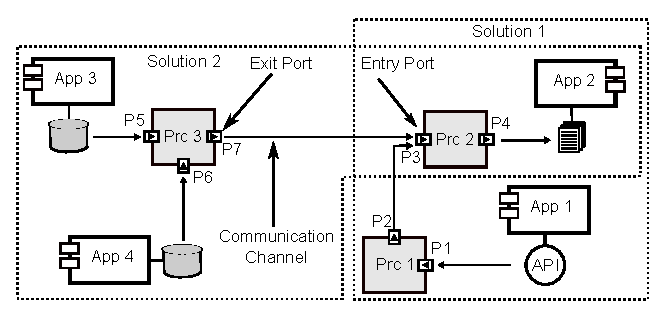
\includegraphics[scale=0.7]{./figs/sample-solution.eps}
%   \caption{Sample EAI solutions.}
%    \label{fig:sample-eai-solution}
%\end{figure}
%-- Context
%A Integração de Aplicações Empresariais (EAI) é o campo de estudo que proporciona metodologias, técnicas e ferramentas para a 
\noindent 
%--Context
As empresas possuem um ecossistema de software composto por diversas aplicações que geralmente são desenvolvidas internamente ou adquiridas de terceiros. O avanço das tecnologias de desenvolvimento de aplicações e a incorporação de serviços de software disponíveis na internet têm deixado os ecossistemas de software ainda mais heterogêneos. Os processos de negócio de uma empresa precisam ser suportados por um conjunto de aplicações e serviços de software que integram seu ecossistema, porém, frequentemente, tais aplicações e serviços não estão preparados para trabalhar de forma conjunta. A Integração de Aplicações Empresariais (EAI) é o campo de estudo que oferece metodologias, técnicas e ferramentas para que os processos de negócio funcionem de forma sincronizada, promovendo repostas rápidas e confiáveis.  

%--Problem
As plataformas de integração são softwares especializados que permitem projetar, executar e monitorar soluções de integração, as quais conectam funcionalidades e dados de diferentes aplicações. Uma solução de integração implementa um fluxo de integração composto por distintas tarefas atômicas que são executadas ao longo desse fluxo. Gregor Hophe e Bobby Woolf~\cite{hohpe2004} documentaram um conjunto de padrões de integração que tem inspirado o desenvolvimento de plataformas de integração de código aberto e que por sua vez organizam o fluxo de integração seguindo uma arquitetura Pipes\&Filters~\cite{alexander1977}. 
%Dentre essas plataformas, destacam-se Camel~\cite{isen2010}, Spring~\cite{fisher2012}, Mule~\cite{dossot2014}, Guaraná~\cite{frantz2016}, Jitterbit~\cite{russell2012} e
% WSO2 ESB~\cite{indrasiri2016}. 
 Usualmente, essas plataformas fornecem uma linguagem de domínio específico, um kit de ferramentas de desenvolvimento, um motor de execução e uma ferramenta de monitoramento. A linguagem de domínio específico possibilita a descrição de modelos conceituais para soluções de integração. O kit de desenvolvimento é um conjunto de ferramentas de software que permite a implementação de soluções, ou seja, transforma uma solução conceitual em código executável. O motor proporciona todo o suporte necessário à execução das soluções de integração. A ferramenta de monitoramento é utilizada para detectar erros que possam ocorrer durante a execução de soluções de integração. O motor é o responsável pela execução das soluções de integração~\cite{frantz2016}. 

As tarefas da solução de integração são executadas por meio de recursos computacionais presentes no motor de execução, dentre os quais estão as \emph{threads} de execução. Neste contexto, as \emph{threads} s\~{a}o usadas para proporcionar que as tarefas sejam executadas de forma simultânea, por meio da programação \emph{multithreads}~\cite{dietel2009,tanebaum2009}. Nesse tipo de programação, a criação de \emph{threads} pode impactar o desempenho da execução de uma solução de integração.

%-- Why it is a problem
Um algoritmo de agendamento de tarefas inadequado aumenta o tempo de execução, impactando o desempenho da solução de integração. A abordagem mais comum é a contratação de mais recursos computacionais, porém essa alternativa é financeiramente onerosa e nem sempre viável. Nossa revisão da literatura identificou que os motores de integração adotam como política de agendamento de tarefas as políticas de prioridade e a \textit{First-In-First-Out} (FIFO). Há propostas de algoritmos de agendamento de tarefas para máquina virtuais em sistemas distribuídos~\cite{rodriguez2014,al2015}, porém não foram identificadas propostas que foquem na otimização de desempenho de motores de execução de plataformas de integração de sistemas. 
%
% O agendamento de fluxo de trabalho tem sido amplamente estudado ao longo dos anos, nos quais os algoritmos se concentram na geração de soluções aproximadas ou quase ótimas, por se tratar de um problema não polinomial difícil~\cite{sousa2004}. Pandey et al.~\cite{pandey2010} propõem um algoritmo baseado em PSO para minimizar o custo de execução de um único fluxo de trabalho enquanto equilibra a carga da tarefa nos recursos disponíveis. Wu et al.~\cite{wu2010} usam PSO para produzir um agendamento quase ideal, se preocupando em minimizar custo e tempo, mas assume que um conjunto limitado de recursos, sem levar em conta a elasticidade proporcionada com a computação em das nuvens. O algoritmo de Byun et al.~\cite{byun2011} estima o número ótimo de recursos que precisam ser alocados para que o custo de execução de um fluxo de trabalho seja minimizado. Sua abordagem aproveita a elasticidade dos recursos da nuvem, mas não considera a natureza heterogênea dos recursos computacionais.

A contribuição deste trabalho é a aplicação da meta-heurística \textit{Particle Swarm Optimization} (PSO) para o contexto dos motores de execução, nos quais as políticas de agendamento adotadas, não consideram o tempo de espera na fila de tarefas prontas, nem a complexidade computacional das tarefas. PSO é fácil de implementar e existirem poucos parâmetros para serem ajustado, adequando-se ao problema de encontrar melhor agendamento das tarefas. Classifica-se como uma pesquisa exploratória, a medida que busca um método mais eficiente do que os existentes, na resolução do problema. Um resumo com ideias iniciais para esse trabalho foi apresentado em um seminário de pesquisa~\cite{sellaro2017}, e o presente artigo as discute de forma mais ampla e completa  a proposta de um algoritmo que busca o mapeamento ótimo das tarefas para os pools de \emph{threads}.

%-- Solution
O resto deste artigo está organizado como segue. A Seção 2 apresenta a formulação do problema. A Seção 3 descreve sucintamente a técnica PSO. A Seção 4 expõe a abordagem proposta. E a Seção 5 apresenta nossas conclusões e perspectivas de trabalhos futuros. 
	%==============================================================================
\section{Related Works}
\label{sec:Trabalhos}
%==============================================================================
Particle swarm optimization has become popular due to its simplicity and its effectiveness in wide range of application with low computational cost. The PSO has also been applied to solve NP-Hard problems~\cite{sousa2004} like scheduling~\cite{veeramachaneni2004,Dasgupta2014} and task allocation~\cite{yin2006, zavala2008}.

Many researches about workflow scheduling problem under the cloud computing environment have used PSO, as mentioned below. Pandey et al.~\cite{pandey2010} seeks to minimize the cost of running a single workflow while balancing the task load on available resources. Wu et al.~\cite{wu2010} is concerned with minimizing cost and time, but assumes that a limited set of resources, without taking into account the elasticity provided by cloud computing. Byun et al.~\cite{byun2011} estimate the optimal number of resources that need to be allocated so that the cost of running a workflow is minimized. Its approach takes advantage of the elasticity of cloud resources, but does not consider the heterogeneous nature of computing resources. Jianfang et al.~\cite{Marcon2013} concern with security requirements in order to avoid the risk  of sensitive  data being  leaked or tampered in the process of transmission or execution. Rodrigues and Buyya~\cite{rodriguez2014} approach cost minimization with the deadline constrained. Yassa et al. aims to minimize energy consumption while preserving the users Quality of Service (QoS) preferences, by using an iterative method called Multi-objective Discrete Particle Swarm Optimization (MODPSO) combined with the Dynamic Voltage and Frequency Scaling (DVFS) technique. 

Particle swarm optimization also has been applied for scheduling tasks in grid environments~\cite{zhang2006, liu2010}. Aron et al.~\cite{aron2015} propose the PSO-based hyper-heuristic method that minimizes the time and cost along with optimized utilization of the resources in the grid environment. Sidhu et al. propose a load rebalance algorithm using PSO together with the smallest position value (SPV) technique for task schedule problem~\cite{sidhu2013}. Ramemezani et al.~\cite{ramezani2014} proposed a Task-based System Load Balancing (TBSLB) that achieves system load balancing by migrating tasks from an overloaded VM to another homogeneous VM, instead of migrating the overloaded VM in its entirety.

    %==============================================================================
\section{Background}
\label{sec:background}
%==============================================================================

%==============================================================================
\subsection{Particle Swarm Optimization}
\label{subsec:PSO}
%==============================================================================
\textit{Particle Swarm Optimization} (PSO) foi introduzido por Kennedy e Eberhart em 1995~\cite{eberhart1995}, e foi inspirado no comportamento social de organismos biológicos, mais especificamente na habilidade de algumas espécies de animais de trabalhar em conjunto para localizar boas regiões com fontes de alimento, assim como ocorre em cardumes e em bandos de pássaros~\cite{bratton2007}. Em outras palavras, é baseado em um enxame de partículas (\emph{Particle Swarm}) que se movem pelo espaço e se comunicam para determinar uma direção de busca ideal. O PSO tem melhor desempenho computacional para este tipo de problema de otimização de funções não-lineares de alta dimensionalidade com variáveis contínuas, do que outros algoritmos~\cite{eberhart1995,bratton2007,alrashidi2009} e tem menos parâmetros para ajustar, facilitando sua implementação. O PSO vem sendo utilizado com sucesso na solução de problemas da ciência e da engenharia devido à sua simplicidade, eficácia e robustez~\cite{fukuyama1999, ourique2002, sousa2004,van2006,engelbrecht2007, alrashidi2009,rodriguez2014,al2015}. Apresenta como desvantagens, a necessidade de informação do tomador de decisão, parâmetros difíceis de ajustar, e ainda incapacidade de alcançar a Frente de Pareto, principalmente em problemas com multimodalidade, aqueles com múltiplas soluções ótimas, onde algumas podem ser melhores soluções globais e outras melhores soluções locais~\cite{figueiredo2013}, porém adapta-se ao problema abordado.

Cada partícula $ i $ do enxame $ S $ é representada por sua posição e sua velocidade. A posição é um vetor de $ n $ dimensões, cujos componentes representam os parâmetros da função objetivo. As partículas controlam a sua melhor posição $ pbest $ e a melhor posição global $ gbest $, a melhor solução conhecida dentro de sua vizinhança.

Inicialmente, as partículas do enxame possuem posições aleatórias no espaço de busca, obedecendo uma distribuição de probabilidade uniforme. Posteriormente, a posição $ {x_i}\left( t \right) $ de cada partícula $ i $ na iteração $ t $ é modificada por uma velocidade estocástica $ {v_i}\left( t \right) $ que depende da distância que a partícula está da sua melhor solução conhecida e da distância para a melhor solução conhecida dentro de sua vizinhança. Cada partícula $i \in S$ se movimenta em cada dimensão $j \in \left\{ {1,2,..n} \right\}$ do espaço de busca em um instante discreto de tempo $ t $, segundo as Equações~\ref{equa:pso1} e~\ref{equa:pso2}:
\begin{equation}
{\overrightarrow x _i}\left( {t + 1} \right) = {\overrightarrow x _{_i}}\left( t \right) + {\overrightarrow v _i}\left( t \right)
\label{equa:pso1}
\end{equation}
%
\begin{equation}
{\overrightarrow v _i}\left( {t + 1} \right) = w{\overrightarrow v _i}\left( t \right) + {c_1}{r_1}\left( {\overrightarrow x _i^*\left( t \right) - {{\overrightarrow x }_{_i}}\left( t \right)} \right) + {c_2}{r_2}\left( {{{\overrightarrow x }^*}\left( t \right) - {{\overrightarrow x }_{_i}}\left( t \right)} \right)
\label{equa:pso2}
\end{equation}
onde:
$ w $ = inércia

$ c _i $ = coeficiente de aceleração, $i=\left( 1,2 \right)$

$ r _i $ = número aleatório pertencente a uma distribuição de probabilidade uniforme , $i=\left( 1,2 \right)$ e ${r_i} \in \left[ {0,1} \right]$

$  \overrightarrow x _i^*\left( t \right) $ = melhor posição da partícula $ i $
	
$ {\overrightarrow x }^*\left( t \right) $ = posição da melhor partícula da população
	
${\overrightarrow x _{_i}}\left( t \right)$ = posição atual da partícula $ i $\\
Quando a vizinhança das partículas consiste no enxame inteiro, a posição ${\overrightarrow x _{_i}}\left( t \right)$ é denominada de $ gbest $. O vetor velocidade é quem orienta o processo de otimização, usando tanto o conhecimento adquirido particularmente pela partícula quanto o conhecimento adquirido pela partícula baseada na interação com sua vizinhança. O termo $ {c_1}{r_1}\left( {\overrightarrow x _i^*\left( t \right) - {{\overrightarrow x }_{_i}}\left( t \right)} \right) $ da equação de atualização da velocidade é a componente cognitiva e representa a experiência da partícula. Essa componente é a responsável pela tendência que a partícula tem de voltar para a melhor solução encontrada por ela no passado. O termo $ {c_2}{r_2}\left( {{{\overrightarrow x }^*}\left( t \right) - {{\overrightarrow x }_{_i}}\left( t \right)} \right) $, por sua vez, é conhecido como componente social da equação da velocidade, e representa o conhecimento coletivo do enxame, sendo responsável por atrair cada partícula para a melhor solução encontrada por alguma partícula de sua vizinhança. 
%A Figura~\ref{fig:grafico-pso} mostra a representação do movimento de uma partícula em um espaço de busca de dimensão igual a 2. 
%\begin{figure}[htb]
%	\centering
%	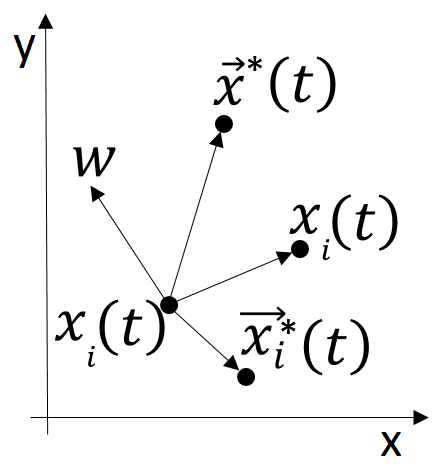
\includegraphics[scale=0.2]{./figs/grafico-pso.png}
%    %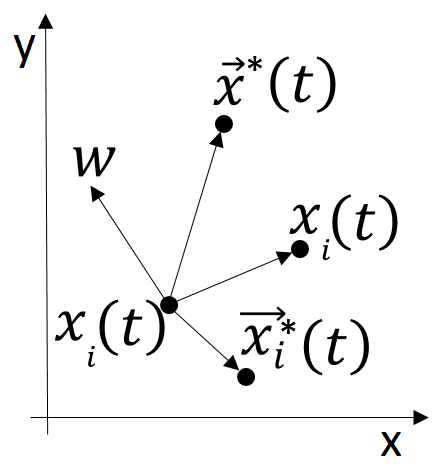
\includegraphics[width=\linewidth]{./figs/grafico-pso.png}
%   \caption{Movimento da partícula em um espaço de busca.}
%    \label{fig:grafico-pso}
%\end{figure}
O vetor velocidade $ \overrightarrow v _i $ é a soma vetorial das componentes cognitiva e social com a inércia da partícula. A inércia $ w $ atua como uma memória da direção da velocidade anterior da partícula e impede que haja alterações bruscas na direção da velocidade partícula~\cite{engelbrecht2007}. Assim, caso a partícula esteja se dirigindo a uma boa região, a descoberta de um novo líder social não alterará completamente essa direção. O papel da componente cognitiva é aproximar a partícula na direção da melhor posição encontrada por ela desde o início da busca. Dessa forma, a partícula deverá encontrar uma boa posição que provavelmente está próxima do seu líder cognitivo atual. Através da componente social, as partículas comunicam a informação sobre as melhores posições encontradas por elas desde o início do processo de busca, sendo considerada como a mais importante componente na equação da velocidade das partículas.

O pseudo-código do PSO é apresentado no Algoritmo~\ref{algoritmo-pso}. A cada passo, o algoritmo irá mudar a velocidade de cada partícula em direção às posições $ pbest $ e $ gbest $, onde a posição e a velocidade da partícula são atualizadas conforme as Equações~\ref{equa:pso1} e~\ref{equa:pso2}, respectivamente. Um termo aleatório $ r $ pondera o quanto a partícula se movimenta em direção a esses valores, onde diferentes números aleatórios são gerados em direção à aceleração para $ pbest $ e $ gbest $ locais~\cite{lazinica2009}. O algoritmo continuará a iterar até que um critério de parada seja alcançado. Geralmente, esse critério de parada é um número máximo de iterações especificado ou um valor aptidão pré-definido considerado bom o suficiente. A equação de velocidade contém vários parâmetros que afetam o desempenho do algoritmo e alguns afetam significativamente na convergência do algoritmo. A inércia $ w $, por exemplo, é fundamental para a convergência do algoritmo. Ela determina o quanto as velocidades anteriores afetarão a velocidade atual e definirá um equilíbrio entre o componente cognitivo local e o global social das partículas. Se o valor da inércia for alto, a velocidade aumentará, favorecendo a busca global. Mas, se o valor for baixo, as partículas sofrerão uma desaceleração, favorecendo a busca local. Dessa forma, um valor $ w $ que equilibra a pesquisa global e local implica menos iterações para que o algoritmo possa convergir.
\begin{algorithm}
	\caption{\textit{Particle Swarm Optimization}}
	\begin{algorithmic}[1]
		\State {$ d  \gets n$} \Comment {Inicializa a dimensão das partículas para $d$}
		\State {$ x[i]  \gets x _{aleatorio}$} \Comment {Inicializa a população de partículas com posições e velocidades aleatórias}
		\ {$ v[i]  \gets v _{aleatorio}$}
		\While {$ criterio parada = falso$} \Comment {Repete enquanto o critério de parada não tiver sido alcançado}
			\For{i}{1}{n} \Comment {Para cada partícula calcula o seu valor aptidão, compara o valor aptidão da partícula com o valor $pbest$ e com o valor de $gbest$}
			
				\If {$x_{atual} \leftrightarrow pbest$} \Comment {Se o valor atual da partícula é melhor do que $pbest$} 
					\State {$ x[i]  \gets x _{atual}$} 
					\ {$ pbest  \gets x _{atual}$}	 
				\EndIf
				\If {$x_{atual} \leftrightarrow gbest$} \Comment {Se o valor atual da partícula é melhor do que $gbest$}  
					\State {$ x[i]  \gets x _{atual}$}	
					\ {$ gbest  \gets x _{atual}$}
				\EndIf	
				
				\State {$ x[i]  \gets x _{calculada}$} \Comment {Atualiza a posição e velocidade da partícula  Equações~\ref{equa:pso1} e~\ref{equa:pso2}}
				
					 \ {$ v[i]  \gets v _{calcculada}$} 	
			\EndFor
		\EndWhile	
	\end{algorithmic}
	\label{algoritmo-pso}
\end{algorithm}
Apesar de $c_1$ e $c_2$ não influenciarem diretamente na convergência do PSO, o ajuste desses parâmetros agiliza e evita que o algoritmo seja pego em mínimos locais. O parâmetro $c_1$ é referido como parâmetro cognitivo e o valor $c_1r_1$, na Equação~\ref{equa:pso2}, define a relevância da melhor posição anterior. $c_2$ é referido como o parâmetro social e $c_2r_2$ e determina o comportamento da partícula em relação a outros vizinhos.

O número, a dimensão das partículas, o alcance e a velocidade máxima das partículas são parâmetros utilizados como entrada para o algoritmo, embora não componham a definição de velocidade. Quanto ao número de partículas, um valor alto costuma aumentar a probabilidade de encontrar o ótimo global. O valor deste número depende da complexidade do problema de otimização, mas um intervalo típico é entre 20 e 40 partículas~\cite {rodriguez2014}. Os valores para a dimensão das partículas e o alcance, no qual sua movimentação é permitida, são determinados unicamente pela natureza do problema que está sendo resolvido e de como ele é modelado para se adequar ao PSO. A velocidade máxima define a mudança máxima que uma partícula pode ter em uma iteração e normalmente seu valor é aproximadamente a metade do alcance de posição da partícula~\cite{rodriguez2014}.

%==============================================================================
\subsection{Runtime System Model}
\label{subsec:runtime}
%==============================================================================
 	%==============================================================================
\section{Problem Formulation}
\label{sec:formulacao_problema}
%==============================================================================
Numa solução de integração, baseada no estilo arquitetural \emph{Pipes\&Filters}~\cite{alexander1977}, os \textit{pipes} são representados por canais de mensagens e os \textit{filters} por tarefas atômicas que implementam um padrão de integração concreto e processam dados encapsulados em mensagens.
% A Figura~\ref{fig:pipes-filters} representa esse estilo arquitetural.
%\begin{figure}[htb]
%	\centering
%	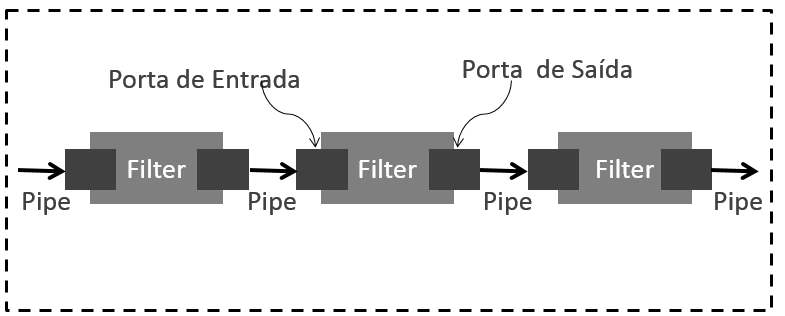
\includegraphics[width=\linewidth]{./figs/pipes_filters.png}
%	\caption{Estilo arquitetural \emph{Pipes\&Filters}}
%	\label{fig:pipes-filters}
%\end{figure}
A Figura~\ref{fig:sample-cafe} mostra o modelo conceitual de uma solução de integração para o problema Café, introduzido por Gregor Hohpe~\cite{hohpe2005} modelado com Guaraná~\cite{frantz2016}.
\begin{figure}[htb]
	\centering
	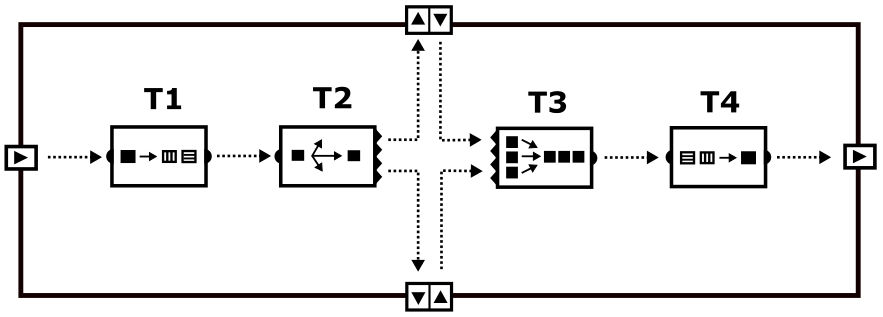
\includegraphics[scale=0.25]{./figs/cafe-guarana.png}
	%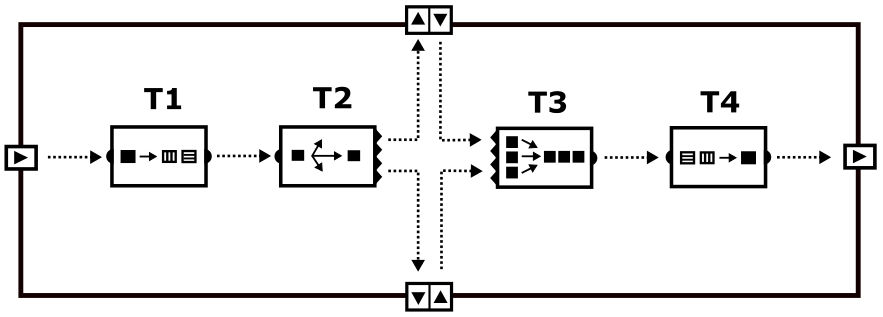
\includegraphics[width=\linewidth]{./figs/cafe-guarana.png}
	\caption{Solução de integração Café}
	%Fonte: \cite{fisher2012spring}
	\label{fig:sample-cafe}
\end{figure}
O modelo conceitual pode ser representado como fluxos de trabalho modelados como Grafos Direcionados Acíclicos, definidos por W(T,E), onde $T = \{t_1,t_2,..t_n\}$ é o conjunto de tarefas e $E$ é o conjunto de arestas direcionadas. Uma aresta $e_{ij}$ da forma $({t_i},{t_j})$ existe, se houver uma dependência de dados entre $t_i$ e $t_j$, onde $t_i$ é tarefa pai de $t_j$ e $t_j$ é tarefa filha de $t_i$. Logo, uma tarefa filha não pode ser executada até que todas as suas tarefas pai estejam concluídas. 
%A Figura~\ref{fig:workflow} mostra fluxos de trabalho da solução de integração Café, onde cada vértice representa uma tarefa e cada aresta possui um peso, que representa o tempo de espera da mensagem na fila de tarefas prontas.
%\begin{figure}[htb]
%	\centering
%	./figs/matrizes-h.pngF
%	%
\includegraphics[width=\linewidth]{./figs/workflow.png}
%	\caption{Workflow da solução de integração Café.}
%	\label{fig:workflow}
%\end{figure}
Considera-se que o motor de execução oferece uma variedade de recursos computacionais para execução das tarefas da solução de integração. Essa variedade de recursos é definida por \emph{pool} de \emph{threads}, com diferentes números de \emph{threads}, onde uma \emph{thread} é a unidade básica de processamento. Assim, assume-se que um motor de execução pode ter mais de um \emph{pool} de \emph{threads} e que o número de \emph{threads} em cada um pode ser diferente, ou seja, um \emph{pool} com uma quantidade \textit{x} \emph{threads} e outro com uma quantidade \textit{y}. Considera-se ainda, que um motor de execução tem uma quantidade limitada de recursos computacionais ${\delta _r}$, sendo um recurso computacional $Pool$, um \emph{pool} de \emph{threads} que tem um tipo $Pool _i$, uma capacidade de processamento $PPool_j$. O tipo diferencia os \emph{pools}, a capacidade de processamento é a quantidade de \emph{threads} do \emph{pool}. A capacidade de memória não é tratada; assume-se que é suficiente para executar as tarefas do fluxo de trabalho. Assume-se que para cada tipo de recurso, a capacidade de processamento é definida em termos de instruções por ciclo (IPC), que pode ser estimada~\cite{abraham2016runtime}. Esta informação é usada no algoritmo, para calcular o tempo de execução de uma tarefa em um determinado \emph{pool} de \emph{threads} $Pool$. A variação do desempenho pode ser modelada pelo ajuste da capacidade do $Pool$ e introduzindo uma degradação de desempenho $deg_{Pool_{j}}$ ~\cite{rodriguez2014}. 
O tempo de execução $TE_{{t_i}}^{Poo{l_j}}$ da tarefa $t_i$ em um $Pool$ de tipo $Pool_j$ é estimado pelo tamanho $Ta{m_{{t_i}}}$ da tarefa em instruções por ciclo (IPC), calculado pela Equação~\ref{equa:tempo-execucao}. 
\begin{equation}
TE_{{t_i}}^{Pool_{j}} = Ta{m_{{t_i}}}/({P_{Pool_{j}}}*(1 - {\deg _{Pool_{j}}}))
\label{equa:tempo-execucao}
\end{equation}
%onde:
%
%$Ta{m_{{t_i}}}$ = tamanho da tarefa
%
%$ {P_{Poo{l_j}}} $ = capacidade de processamento do \emph{pool} de threads
%
%$ {\deg _{Poo{l_j}}} $ = degradação de desempenho
O tempo médio de espera na fila de tarefas $TF{i_{e_{ij}}}$ é definido como o tempo para transferir dados entre uma tarefa pai $t_i$ e sua tarefa filha $t_j$ e assume-se que ele pode ser monitorado e medido.  

Finalmente, o tempo total de processamento $TP_{{t_i}}^{Poo{l_j}}$ de uma tarefa em um $Pool$ é calculado na Equação~\ref{equa:tempo-processamento}, onde k é o número de arestas, $t_i$ é uma tarefa pai e $s_k$ representa o tempo gasto pelo motor na troca de \emph{pool} de threads, de maneira que $s_k$ = 0, quando $t_i$ e $t_j$ são processadas no mesmo \emph{pool} e  $s_k$ = 1, caso contrário.
\begin{equation}
TP_{{t_i}}^{Poo{l_j}} = TE_{{t_i}}^{Poo{l_j}} + (\sum\limits_1^k {T{F_{ij}} + {s_k}} )
\label{equa:tempo-processamento}
\end{equation}
%onde:
%
%$ TE_{{t_i}}^{Poo{l_j}} $ = tempo de execução da tarefa em um determinado \emph{pool} de threads.
%
%$TF{i_{e_ij}}$  = tempo de espera na fila de tarefas, ou seja, tempo que para transferir dados entre uma tarefa e sua tarefa filha. 
%
%$ {s_k} $ = tempo gasto na troca de \emph{pool} de threads.
%
%$ k $ =  número de arestas em que uma tarefa é uma tarefa pai. 
O objetivo é encontrar um agendamento de tarefas que possibilite executar as tarefas da solução de integração em \emph{pools} de \emph{threads} do motor de execução, minimizando o tempo total de execução e sem aumentar a quantidade de recursos computacionais. O agendamento de tarefas é definido por $A= (R, M, TR, TTE)$, sendo $R$ um conjunto de recursos; $M$ o mapeamento de tarefas em recursos, $TR$, $TR=\arrowvert R\arrowvert =n$, o total de recursos, $TTE$ o tempo total de execução. Um exemplo é mostrado na Figura~\ref{fig:grafico-mapeamento}, representando o agendamento para o fluxo de trabalho, em que cada uma das quatro tarefas é mapeada para ser executada por um dos três recursos disponíveis, e onde as tarefas pais são executadas antes das sua tarefas filhas, mantendo assim a dependência dos dados.
\begin{figure}[htb]
	\centering
	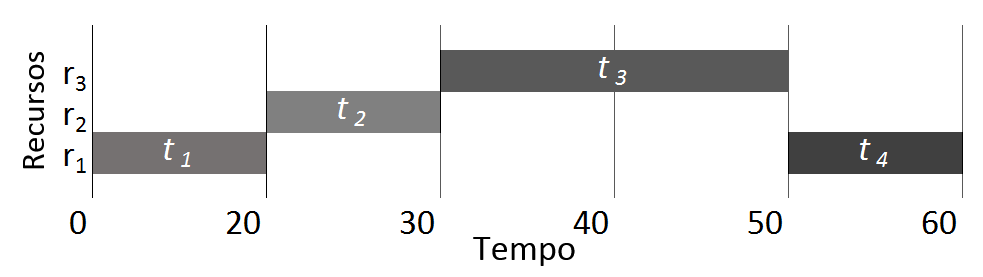
\includegraphics[scale=0.2]{./figs/grafico-mapeamento.png}
	%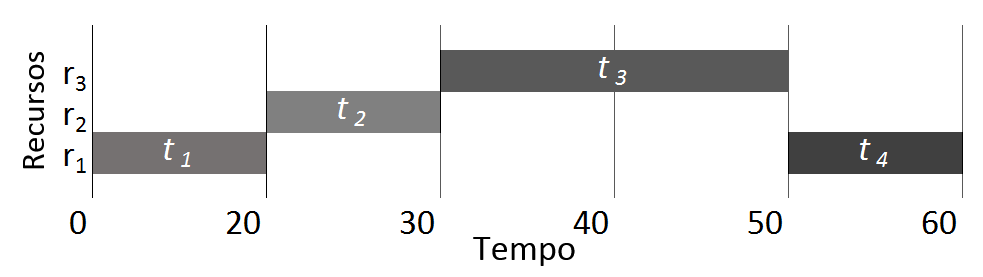
\includegraphics[width=\linewidth]{./figs/grafico-mapeamento.png}
	\caption{Agendamento para o workflow do Café.}
	\label{fig:grafico-mapeamento}
\end{figure}
$R = \{ {r_1},{r_2},...,{r_n}\}$  é o conjunto de recursos (\emph{pools} de \emph{threads}) do motor de execução, onde cada recurso $r_i$ tem associado a ele um $Pool$ do tipo $Pool_i$, um tempo de início estimado para alocação do recurso estimado ${TIni_{r_i}}$. e um tempo de finalização estimado ${TFim_{r_i}}$. M representa um mapeamento para cada uma das tarefas do fluxo de trabalho e é constituído por tuplas $ m_{{t_i}}^{{r_j}} = ({t_i},{r_j},TIn{i_{{t_i}}},TFi{n_{{t_i}}})$, significando que a tarefa $t_i$ será executada pelo recurso $r_j$, com o início da execução agendado para $ TIn{i_{{t_i}}} $ e previsão de término em $ TFi{n_{{t_i}}} $. A Equação~\ref{equa:tempo-total-execução} mostra como o tempo total de execução $ TTE $ é calculado:
\begin{equation}
TTE = \max \{ TFi{m_{{t_i}}}:{t_i} \in T\} 
\label{equa:tempo-total-execução}
\end{equation}
Assim, o problema pode ser formulado como: \textit{encontrar um agendamento $A$ com o menor tempo total de execução $TTE$ da solução de integração, sem exceder um valor pré-definido para o total de recursos $TR$}. Essa formulação é representada pela Equação~\ref{equa:problema}:
\begin{equation}
Minimize {TTE} 
\label{equa:problema}
\end{equation}
\begin{center}
	 sujeito a ${TR \le {\delta _r}} $
\end{center}

% 	%==============================================================================
\section{Particle Swarm Optimization}
\label{sec:PSO}
%==============================================================================
\textit{Particle Swarm Optimization} (PSO) foi introduzido por Kennedy e Eberhart em 1995~\cite{eberhart1995}, e foi inspirado no comportamento social de organismos biológicos, mais especificamente na habilidade de algumas espécies de animais de trabalhar em conjunto para localizar boas regiões com fontes de alimento, assim como ocorre em cardumes e em bandos de pássaros~\cite{bratton2007}. Em outras palavras, é baseado em um enxame de partículas (\emph{Particle Swarm}) que se movem pelo espaço e se comunicam para determinar uma direção de busca ideal. O PSO tem melhor desempenho computacional para este tipo de problema de otimização de funções não-lineares de alta dimensionalidade com variáveis contínuas, do que outros algoritmos~\cite{eberhart1995,bratton2007,alrashidi2009} e tem menos parâmetros para ajustar, facilitando sua implementação. O PSO vem sendo utilizado com sucesso na solução de problemas da ciência e da engenharia devido à sua simplicidade, eficácia e robustez~\cite{fukuyama1999, ourique2002, sousa2004,van2006,engelbrecht2007, alrashidi2009,rodriguez2014,al2015}. Apresenta como desvantagens, a necessidade de informação do tomador de decisão, parâmetros difíceis de ajustar, e ainda incapacidade de alcançar a Frente de Pareto, principalmente em problemas com multimodalidade, aqueles com múltiplas soluções ótimas, onde algumas podem ser melhores soluções globais e outras melhores soluções locais~\cite{figueiredo2013}, porém adapta-se ao problema abordado.

Cada partícula $ i $ do enxame $ S $ é representada por sua posição e sua velocidade. A posição é um vetor de $ n $ dimensões, cujos componentes representam os parâmetros da função objetivo. As partículas controlam a sua melhor posição $ pbest $ e a melhor posição global $ gbest $, a melhor solução conhecida dentro de sua vizinhança.

Inicialmente, as partículas do enxame possuem posições aleatórias no espaço de busca, obedecendo uma distribuição de probabilidade uniforme. Posteriormente, a posição $ {x_i}\left( t \right) $ de cada partícula $ i $ na iteração $ t $ é modificada por uma velocidade estocástica $ {v_i}\left( t \right) $ que depende da distância que a partícula está da sua melhor solução conhecida e da distância para a melhor solução conhecida dentro de sua vizinhança. Cada partícula $i \in S$ se movimenta em cada dimensão $j \in \left\{ {1,2,..n} \right\}$ do espaço de busca em um instante discreto de tempo $ t $, segundo as Equações~\ref{equa:pso1} e~\ref{equa:pso2}:
\begin{equation}
{\overrightarrow x _i}\left( {t + 1} \right) = {\overrightarrow x _{_i}}\left( t \right) + {\overrightarrow v _i}\left( t \right)
\label{equa:pso1}
\end{equation}
%
\begin{equation}
{\overrightarrow v _i}\left( {t + 1} \right) = w{\overrightarrow v _i}\left( t \right) + {c_1}{r_1}\left( {\overrightarrow x _i^*\left( t \right) - {{\overrightarrow x }_{_i}}\left( t \right)} \right) + {c_2}{r_2}\left( {{{\overrightarrow x }^*}\left( t \right) - {{\overrightarrow x }_{_i}}\left( t \right)} \right)
\label{equa:pso2}
\end{equation}
onde:
$ w $ = inércia

$ c _i $ = coeficiente de aceleração, $i=\left( 1,2 \right)$

$ r _i $ = número aleatório pertencente a uma distribuição de probabilidade uniforme , $i=\left( 1,2 \right)$ e ${r_i} \in \left[ {0,1} \right]$

$  \overrightarrow x _i^*\left( t \right) $ = melhor posição da partícula $ i $
	
$ {\overrightarrow x }^*\left( t \right) $ = posição da melhor partícula da população
	
${\overrightarrow x _{_i}}\left( t \right)$ = posição atual da partícula $ i $\\
Quando a vizinhança das partículas consiste no enxame inteiro, a posição ${\overrightarrow x _{_i}}\left( t \right)$ é denominada de $ gbest $. O vetor velocidade é quem orienta o processo de otimização, usando tanto o conhecimento adquirido particularmente pela partícula quanto o conhecimento adquirido pela partícula baseada na interação com sua vizinhança. O termo $ {c_1}{r_1}\left( {\overrightarrow x _i^*\left( t \right) - {{\overrightarrow x }_{_i}}\left( t \right)} \right) $ da equação de atualização da velocidade é a componente cognitiva e representa a experiência da partícula. Essa componente é a responsável pela tendência que a partícula tem de voltar para a melhor solução encontrada por ela no passado. O termo $ {c_2}{r_2}\left( {{{\overrightarrow x }^*}\left( t \right) - {{\overrightarrow x }_{_i}}\left( t \right)} \right) $, por sua vez, é conhecido como componente social da equação da velocidade, e representa o conhecimento coletivo do enxame, sendo responsável por atrair cada partícula para a melhor solução encontrada por alguma partícula de sua vizinhança. 
%A Figura~\ref{fig:grafico-pso} mostra a representação do movimento de uma partícula em um espaço de busca de dimensão igual a 2. 
%\begin{figure}[htb]
%	\centering
%	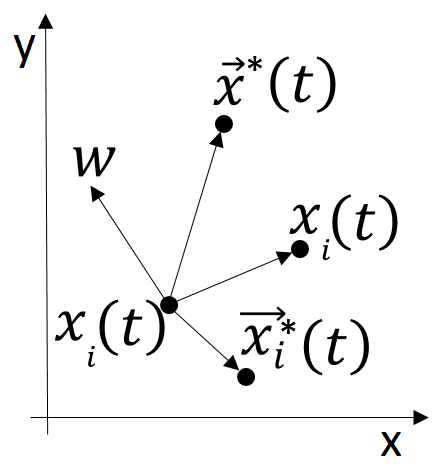
\includegraphics[scale=0.2]{./figs/grafico-pso.png}
%    %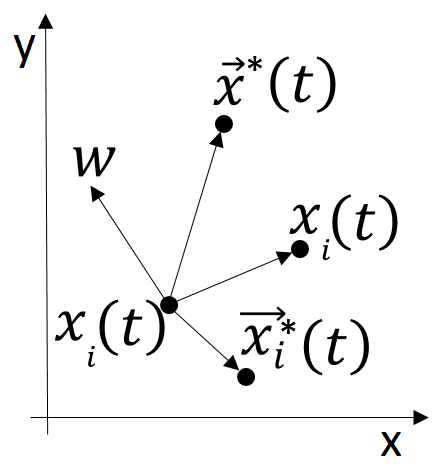
\includegraphics[width=\linewidth]{./figs/grafico-pso.png}
%   \caption{Movimento da partícula em um espaço de busca.}
%    \label{fig:grafico-pso}
%\end{figure}
O vetor velocidade $ \overrightarrow v _i $ é a soma vetorial das componentes cognitiva e social com a inércia da partícula. A inércia $ w $ atua como uma memória da direção da velocidade anterior da partícula e impede que haja alterações bruscas na direção da velocidade partícula~\cite{engelbrecht2007}. Assim, caso a partícula esteja se dirigindo a uma boa região, a descoberta de um novo líder social não alterará completamente essa direção. O papel da componente cognitiva é aproximar a partícula na direção da melhor posição encontrada por ela desde o início da busca. Dessa forma, a partícula deverá encontrar uma boa posição que provavelmente está próxima do seu líder cognitivo atual. Através da componente social, as partículas comunicam a informação sobre as melhores posições encontradas por elas desde o início do processo de busca, sendo considerada como a mais importante componente na equação da velocidade das partículas.

O pseudo-código do PSO é apresentado no Algoritmo~\ref{algoritmo-pso}. A cada passo, o algoritmo irá mudar a velocidade de cada partícula em direção às posições $ pbest $ e $ gbest $, onde a posição e a velocidade da partícula são atualizadas conforme as Equações~\ref{equa:pso1} e~\ref{equa:pso2}, respectivamente. Um termo aleatório $ r $ pondera o quanto a partícula se movimenta em direção a esses valores, onde diferentes números aleatórios são gerados em direção à aceleração para $ pbest $ e $ gbest $ locais~\cite{lazinica2009}. O algoritmo continuará a iterar até que um critério de parada seja alcançado. Geralmente, esse critério de parada é um número máximo de iterações especificado ou um valor aptidão pré-definido considerado bom o suficiente. A equação de velocidade contém vários parâmetros que afetam o desempenho do algoritmo e alguns afetam significativamente na convergência do algoritmo. A inércia $ w $, por exemplo, é fundamental para a convergência do algoritmo. Ela determina o quanto as velocidades anteriores afetarão a velocidade atual e definirá um equilíbrio entre o componente cognitivo local e o global social das partículas. Se o valor da inércia for alto, a velocidade aumentará, favorecendo a busca global. Mas, se o valor for baixo, as partículas sofrerão uma desaceleração, favorecendo a busca local. Dessa forma, um valor $ w $ que equilibra a pesquisa global e local implica menos iterações para que o algoritmo possa convergir.
\begin{algorithm}
	\caption{\textit{Particle Swarm Optimization}}
	\begin{algorithmic}[1]
		\State {$ d  \gets n$} \Comment {Inicializa a dimensão das partículas para $d$}
		\State {$ x[i]  \gets x _{aleatorio}$} \Comment {Inicializa a população de partículas com posições e velocidades aleatórias}
		\ {$ v[i]  \gets v _{aleatorio}$}
		\While {$ criterio parada = falso$} \Comment {Repete enquanto o critério de parada não tiver sido alcançado}
			\For{i}{1}{n} \Comment {Para cada partícula calcula o seu valor aptidão, compara o valor aptidão da partícula com o valor $pbest$ e com o valor de $gbest$}
			
				\If {$x_{atual} \leftrightarrow pbest$} \Comment {Se o valor atual da partícula é melhor do que $pbest$} 
					\State {$ x[i]  \gets x _{atual}$} 
					\ {$ pbest  \gets x _{atual}$}	 
				\EndIf
				\If {$x_{atual} \leftrightarrow gbest$} \Comment {Se o valor atual da partícula é melhor do que $gbest$}  
					\State {$ x[i]  \gets x _{atual}$}	
					\ {$ gbest  \gets x _{atual}$}
				\EndIf	
				
				\State {$ x[i]  \gets x _{calculada}$} \Comment {Atualiza a posição e velocidade da partícula  Equações~\ref{equa:pso1} e~\ref{equa:pso2}}
				
					 \ {$ v[i]  \gets v _{calcculada}$} 	
			\EndFor
		\EndWhile	
	\end{algorithmic}
	\label{algoritmo-pso}
\end{algorithm}
Apesar de $c_1$ e $c_2$ não influenciarem diretamente na convergência do PSO, o ajuste desses parâmetros agiliza e evita que o algoritmo seja pego em mínimos locais. O parâmetro $c_1$ é referido como parâmetro cognitivo e o valor $c_1r_1$, na Equação~\ref{equa:pso2}, define a relevância da melhor posição anterior. $c_2$ é referido como o parâmetro social e $c_2r_2$ e determina o comportamento da partícula em relação a outros vizinhos.

O número, a dimensão das partículas, o alcance e a velocidade máxima das partículas são parâmetros utilizados como entrada para o algoritmo, embora não componham a definição de velocidade. Quanto ao número de partículas, um valor alto costuma aumentar a probabilidade de encontrar o ótimo global. O valor deste número depende da complexidade do problema de otimização, mas um intervalo típico é entre 20 e 40 partículas~\cite {rodriguez2014}. Os valores para a dimensão das partículas e o alcance, no qual sua movimentação é permitida, são determinados unicamente pela natureza do problema que está sendo resolvido e de como ele é modelado para se adequar ao PSO. A velocidade máxima define a mudança máxima que uma partícula pode ter em uma iteração e normalmente seu valor é aproximadamente a metade do alcance de posição da partícula~\cite{rodriguez2014}.
	%==============================================================================
\section{Algorithm}
\label{sec:algoritmo}
%==============================================================================

%==============================================================================
\subsection{Complexity Analysis}
\label{subsec:complexity}
%====================================================================

%==============================================================================
\subsection{Proposal}
\label{subsec:proposal}
%==============================================================================
A modelagem de um problema PSO é dividida em duas fases: definição do problema e definição da função aptidão. A primeira consiste em definir como o problema será codificado, ou seja, definir como a solução será representada. A segunda, em definir o quão \textit{boa} uma partícula será medida, ou seja, definir a função de aptidão.
Já para transformar o problema PSO em um algoritmo, é preciso definir a partícula e sua dimensão. Na abordagem adotada neste artigo, uma partícula representa um fluxo de trabalho e suas tarefas, e dimensão da partícula representa o número de tarefas no fluxo de trabalho. A dimensão de uma partícula serve para localizar sua posição no espaço, definindo o sistema de coordenadas. No exemplo do workflow do Café, a dimensão da partícula é quatro, sendo sua posição especificada por um sistema com quatro coordenadas.

Uma partícula movimenta-se num espaço limitado, denomina-se alcance. Na abordagem adotada neste artigo, o alcance é determinado pelo número de \emph{pools} de \emph{threads} disponíveis para executar a tarefa. Assim, o valor de uma coordenada no sistema de coordenadas, que define o espaço de movimentação da partícula, tem um alcance de 0 até o número máximo de \emph{pools} de \emph{threads} disponíveis. A parte inteira do valor de uma coordenada na posição de uma partícula corresponde ao número de \emph{pools} de \emph{threads} e representa o recurso computacional atribuído a uma tarefa definida por essa coordenada específica. Assim, a posição da partícula corresponde a um mapeamento da tarefa em recursos. 

Para o workflow do Café, valores para as quatro coordenadas(tarefas) do nosso sistema de coordenadas, no qual existem três recursos computacionais (\emph{pools} de \emph{threads} disponíveis), de forma que o valor de cada coordenada poderá variar entre 0 e 3. Há 4 tarefas para serem mapeadas, o que corresponde a dimensão 4 da partícula, portanto a posição da partícula terá 4 coordenadas. O índice da coordenada (de 1 a 4) corresponde a uma tarefa (de $t_1$ a $t_{4}$). O valor da coordenada é um número real de 0 a 3 , correspondendo ao número de recursos disponíveis para cada tarefa, com o máximo de 3 no nosso exemplo. Quando esse número inteiro é arredondado, é determinado o número de recursos disponíveis para cada tarefa. 
%Conforme o exemplo da Figura~\ref{fig:coordenadas}, a coordenada 1 da tarefa 1 tem valor igual a $1,3$ significando que para essa tarefa foi alocado 1 recurso, pois 1 é a parte inteira desse valor; a coordenada 2, corresponde a tarefa 2, tem valor de $ 2,0 $ indica que para a tarefa 2 foram alocados 2 recursos; e assim, sucessivamente até a coordenada 4.
%\begin{figure}[htb]
%\centering
%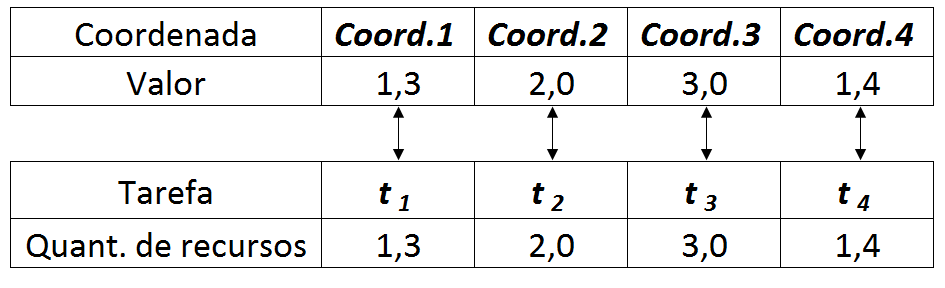
\includegraphics[scale=0.25]{./figs/coordenadas.png}
%\caption{Coordenadas da posição das partículas no espaço.}
%\label{fig:coordenadas}
%\end{figure}
A função de aptidão deve refletir os objetivos do problema de agendamento, pois ela é usada para determinar o quão boa uma determinada solução é. Nessa abordagem, ela é minimizada e seu valor será o tempo total de execução $TTE$ contido no agendamento $A$ derivado da posição da partícula. Considerando que o motor de execução é capaz de aumentar elástica e dinamicamente a quantidade de recursos, o modelo de aquisição oferecido pela computação em nuvem parece ilimitado, ou seja, não há um conjunto de recursos disponíveis que pode ser usado no algoritmo. A estratégia é definir um conjunto inicial de recursos que o algoritmo pode usar para explorar diferentes soluções e alcançar o agendamento. O tamanho desse conjunto será nossa restrição ${TR \le {\delta _r}} $, conforme a Equação~\ref{equa:problema}. Tal estratégia tem de refletir a heterogeneidade dos \emph{pools} de \emph{threads} (diferentes números de \emph{threads}) e oferecer opções suficientes de PSO, a fim de que seja produzida uma partícula adequada, ou seja, a solução. O conjunto de recursos inicial e limitado conterá os recursos que podem ser usados. Se esse conjunto é muito grande, o número de agendamento possíveis aumentará, assim como, o espaço de pesquisa explorado pelo PSO, tornando difícil para o algoritmo convergir e encontrar uma solução adequada~\cite{rodriguez2014}.

Para reduzir o tamanho do espaço de pesquisa, o qual será usado pelo PSO para encontrar um agendamento próximo do ótimo, considera-se um conjunto de recursos inicial $R_{inicial}$, composto por um $Pool$ de cada tipo, para cada tarefa em P; onde P é o conjunto que contém o número máximo de tarefas que podem ser executadas em paralelo para um dado fluxo de trabalho. O algoritmo selecionará o número e o tipo apropriados de $Pools$ para o motor de execução, dentro das opções contidas em $R_{inicial}$. Assim, reflete-se a heterogeneidade dos recursos computacionais e reduz-se o tamanho do espaço de busca, além de permitir mapear todas as tarefas que podem ser executadas em paralelo. O tamanho de $R_{inicial}$ seria igual a $\left| P \right|*n$, onde $n$ é o número de tipos de $Pools$ disponíveis, sendo ainda possível, que o PSO selecione mais de um recurso $\left| P \right|$, se necessário (a menos que $n = 1$).

O problema abordado possui a restrição  ${TR \le {\delta _r}} $, utiliza-se uma versão do PSO que incorpora uma estratégia para tratar restrições~\cite{deb2002}. Nela, sempre que duas soluções estão sendo comparadas e (\textit{i}) ambas as soluções forem viáveis, então a solução com melhor aptidão é selecionada; (\textit{ii}) se uma solução é viável e a outra não é, então a viável é selecionada; e finalmente, (\textit{iii}) se ambas as soluções são inviáveis, aquela que violar menos a restrição é selecionada. No último caso, implica que uma medida de quanto uma solução viola a restrição precisa ser encontrada. O problema define o valor de violação de restrição de uma solução $\delta_k $, a restrição pode ser atribuída a limitação de recursos que se deseja contratar na computação em nuvem ou simplesmente e a quantidade de \emph{threads} físicas das máquinas que irão ser utilizadas na execução da solução de integração. Uma solução do PSO que utilize recursos próximos de $\delta_k$ será preterida em relação a uma solução menos recursos.

O Algoritmo~\ref{algoritmo-agendamento} apresenta o pseudo-código para mapear a posição de uma partícula em um agendamento. O conjunto de recursos $R$ para serem alocados e o conjunto de mapeamentos $M$ de tarefas para recursos são inicializados sem elementos, ou seja, vazios, e tempo total de execução $TTE$ é inicializado com o valor zero. Na sequência, o algoritmo estima o tempo de execução de cada tarefa do fluxo de trabalho para todo o recurso ${r_i} \in {R_{inicial}}$. A representação é uma matriz em que as linhas representam as tarefas, as colunas representam os recursos e a entrada $ TempoExec[i,j] $ corresponde ao tempo gasto para executar a tarefa $t_i$ no recurso $r_j$, calculado conforme a Equação~\ref{equa:tempo-execucao}. O próximo passo é o cálculo ou atribuição da matriz de tempo de transferência de dados, ou tempo de espera na fila de tarefas, o qual assume-se que está sendo obtido por um procedimento, não tratado nesse trabalho, tal como por uma ferramenta de monitoramento. Essa matriz é representada como uma matriz de adjacência ponderada do workflow DAG, onde a entrada $ TempoTransfer[i, j]$ contém o tempo que leva para transferir os dados de saída da tarefa $t_i$ para a tarefa $t_j$ e esse valor é zero sempre que $i =j$ ou não há aresta direcionada conectando $t_i$ (tarefa pai) e $t_j$ (tarefa filha). 
%A Figura~\ref{fig:matrizes} exemplifica essas matrizes para o workflow do Café.
%\begin{figure}[htb]
%	\centering
%	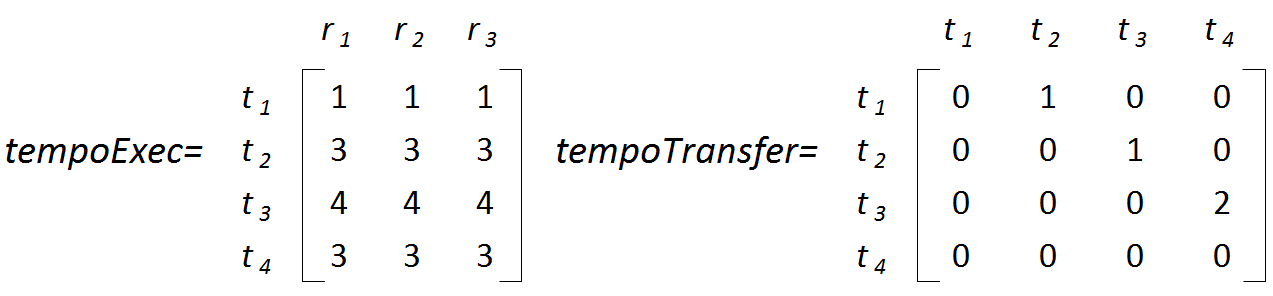
\includegraphics[scale=0.2]{./figs/matrizes-h.png}
%	%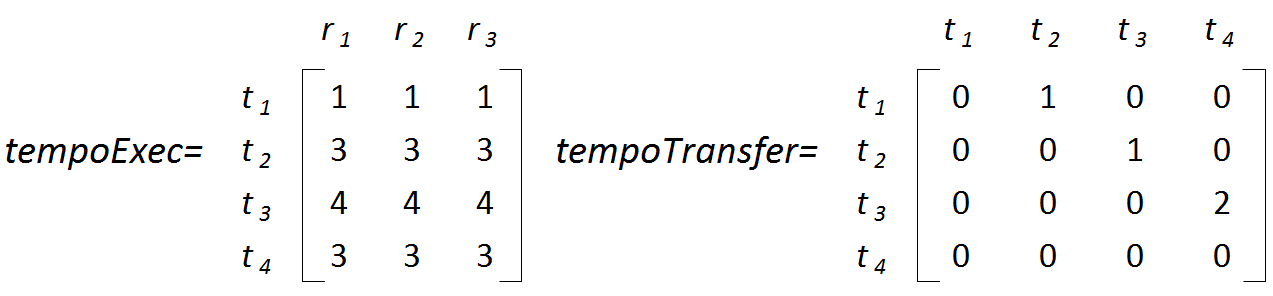
\includegraphics[width=\linewidth]{./figs/matrizes-h.png}
%	\caption{Matrizes Tempo de Execução e de Transferência.}
%	\label{fig:matrizes}
%\end{figure}
De posse dessas informações, o algoritmo inicia determinando a posição da partícula e construindo o agendamento. Para isso, itera para toda $ i $ do \textit{array} de posição $pos$ e atualiza $ R $ e $ M $. Primeiro, determina a tarefa e o recurso que está associado à coordenada atual e seu valor. A estratégia usada para isso é a descrita anteriormente, a qual indica que a coordenada $ i $ corresponde à tarefa $t_i$ e seu valor $pos[i]$ corresponde ao recurso $  {r_{pos[i]}} \in {R_{inicial}} $. Encontrados os componentes, $ {t_i} $ e $ {r_j} $, de uma tupla de mapeamento $ m_{{t_i}}^{{r_j}} $, o algoritmo calcula os demais, o tempo de inicio $ TIn{i_{{t_i}}} $ e tempo de finalização $TFi{n_{{t_i}}}$ da tarefa.

O valor de tempo de início $ TIn{i_{{t_i}}} $ diferencia-se em duas situações. Na primeira, a tarefa não tem tarefa pai e, portanto, pode começar a ser executada, assim que o recurso alocado para ela $r_{pos[i]}$ estiver disponível, o que ocorrerá quando o referido recurso terminar a execução que estiver em andamento. Na segunda situação, a tarefa tem um ou mais pais e, nesse caso, além de esperar que o recurso para ela alocado esteja disponível, também terá que aguardar pelo término da execução das suas tarefas pai, além do tempo de transferência dos dados.

O valor de $TFin_{t_i}$ é calculado baseado no tempo total de processamento e no tempo de início da tarefa. Para determinar o tempo de processamento $TP_{{t_i}}^{r_{pos[j]}}$, é necessário calcular o tempo de execução e o tempo de transferência. O primeiro é $TempoExec[i,pos[i]]$, enquanto o último é calculado pela soma dos valores do tempo de transferência $TempoTransf[i,filha(i)]$ para toda tarefa filha $t_{filha(i)}$ de ${t_i}$, que está mapeada para rodar em um recurso diferente de $r_{pos[i]}$. Esses dois valores são então somados para obter $TP_{{t_i}}^{r_{pos[j]}}$, como definido na Equação~\ref{equa:tempo-processamento}. Por fim, o valor de $TFin_{t_i}$ é obtido pela subtração de $TIni_{t_i}$ de $TP_{{t_i}}^{r_{pos[j]}}$.
Calculados os elementos de $ m $, adiciona-se recurso para $R$, se necessário. 
Quando o algoritmo termina de processar, cada coordenada do vetor posição, $R$ conterá todos os recursos necessários e os tempos de início e finalização. Além disso, o mapeamento completo das tarefas para os recursos estará em $M$ e cada tarefa terá um recurso atribuído a ela e o tempo estimado de início e o de término. Com essas informações o algoritmo pode calcular o $TTE$  associado a solução atual, conforme Equação~\ref{equa:tempo-processamento}. Nesse ponto, o algoritmo calculou $R$, $M$ e $TTE$ e poderá construir e apresentar o agendamento associado para essa posição da partícula.
\begin{algorithm}
	\caption{Geração de agendamento}
	\ {\textbf{Entrada:} Conjunto de fluxo de trabalho de tarefas $ T $}
	
	\ {Conjunto Inicial de recursos $ R_{inicial} $}
	
	\ {Um array  $pos[{\left| T \right|}]$ representando a posição da partícula}
	
	\ {\textbf{Saída:} Um agendamento $ A $}
	
	\begin{algorithmic}[1]
		
		\State { $ \texttt{R} = \emptyset, \texttt{M} =  \emptyset, TTE = 0 $ } \Comment {Inicializa componentes}
		\State { Calcula $ {{TempoExec[}}\left| T \right| \times \left| {{R_{inicial}}} \right|] $}
		\State { Calcula $ {{TempoTransf[}}\left| T \right| \times \left| T \right|] $}
		\For{$ i $}{0}{$\left| T \right|-1$} 
		\State {$ t_i = T[i], r_{pos[i]} = \texttt{R}_{inicial}[pos[i]]  $}
		\If {$ {t_i}$ não tem pai}
		\State {$ TIni_{t_i} = TFin_{r_{pos[i]}} $}
		\Else
		\State {$ TIni_{t_i} = (\max {\{TFin_{t_{pai}}:t_{pai}[ \in pais(t_i) \}},TFin_{r_{pos[i]}}) $}	
		\EndIf
		\State {$ exe = tempoExec \left[ i \right]\left[ {pos\left[ i \right]} \right] $}
		\For {cada filha $ t_{filha} $ de $ t_i $}
		\If {$ t_{filha}$ é mapeada para um recurso diferente de  $r_{pos[i]} $}
		\State { $ trasfer+ = TempoTransf[i][c] $}	
		\EndIf	
		\EndFor
		\State {$TP_{{t_i}}^{r_{pos[j]}} = exe + transf$}
		\State {$ TFin_{t_i} = TP_{{t_i}}^{r_{pos[j]}} - TIni_{t_i}  $}
		\State {$ m_{{t_i}}^{{r_{pos[j]}}} = (t_i,r_{pos[i]},TIni_{t_i},TFin_{t_i})  $}
		\State {$ \texttt{M} = \texttt{M} \cup \{ m_{{t_i}}^{{r_{pos[i]}}}\}   $}
		\If {$ {r_{pos[i]}} \notin \texttt{R}  $}
		\State {$ \texttt{R} = \texttt{R} \cup {r_{pos[i]}}  $}
		\EndIf
		\EndFor 
		\State { Calcula $ TTE $ conforme Equação~\ref{equa:tempo-total-execução} }
		\State {$ A = (R, M, TR, TTE) $}
	\end{algorithmic}
	\label{algoritmo-agendamento}
\end{algorithm}
Finalmente, os Algoritmos~\ref{algoritmo-pso} e \ref{algoritmo-agendamento} são combinados para o agendamento próximo de ótimo. Na linha 4 do Algoritmo~\ref{algoritmo-pso}, em vez de calcular o valor de aptidão da partícula, gera-se o agendamento, conforme Algoritmo~\ref{algoritmo-agendamento}. Em seguida, usa-se o $ TTE $ como valor de aptidão nas etapas seguintes e é introduzido o mecanismo de manipulação de restrição, tal que  ${TR \le {\delta _r}} $.  
	%==============================================================================
\section{Experiments}
\label{sec:experiments}
%==============================================================================
% This section presents the case study experiment. First, we describe the environment in which the experiment was carried out and present the scenarios used, the observed variables. Next, we describe the current task scheduling model and the results obtained with this model. In the same way, we describe the proposed model for optimization of the scheduling of tasks and the results obtained. Finally, we compare and discuss the results obtained in each case.
Esta seção apresenta os experimentos realizados para aferição do desempenho do processamento de mensagens no processo de integração com o modelo proposto, que utiliza múltiplos pools com um número de threads ótimo ou próximo de ótimo, obtidos pelo algoritmo baseado no PSO. O experimento compara os resultados obtidos com o modelo proposto e os resultados obtidos com o modelo tradicional que utiliza um único pool e adota a política FIFO para agendamento do processamento das mensagens pela execução das tarefas. 

Primeiro, descrevemos o ambiente em que o experimento foi realizado, apresentamos os cenários utilizados e as variáveis observadas. Em seguida, descrevemos o modelo de tradicional e os resultados obtidos com este modelo. Do mesmo modo, descrevemos o modelo proposto e os resultados obtidos. Finalmente, comparamos e discutimos esses resultados.
%==============================================================================
\subsection{Environments}
\label{subsec:enviroments}
%==============================================================================
Para implementação dos algoritmos e testes primários, foi utilizado computador com sistema operacional Microsoft Windows 10 Education, Intel (R) Core (TM) i5-5200U CPU, 2.20 GHz; 2195 Mhz, 2 núcleos, 4 processadores lógicos, memória RAM de 4.00 GB.

Já para as experimentações computacionais de alto desempenho, com taxa de entrada de mensagens acima de ... e processos de integração acima de ... tarefas, foi utilizado um servidor com a seguinte configuração: armazenamento SAS de 6 Gb, 12 unidades de 2U, dois controladores de cache de 4 GB; seis discos de 2TB, 2.7 K rpm, NLSAS 12Gbps; cache Intel Xeon E5-4610 v4 1.8GHz de 25M, QPI de 6.4 GT / s, sem turbo, HT, dez núcleos / vinte segmentos; três discos SAS 2.5, 12Gbps de 300GB; vinte e quatro pentes de memória RDIMM de 16 GB, 2400 MT / s; RAID5 com três a seis discos; duas fontes de alimentação redundantes.

De modo similar, utilizou-se o software Matlab~\cite{leonard1995}, versão R2013, para criar e testar os programas, os quais foram posteriormente implementados na linguagem Java, versão ...
Para geração de gráficos e tabelas e dados estatísticos, utilizou-se o software Excel, do pacote Microsoft Office 2016.
%==============================================================================
\subsection{Description}
\label{subsec:description}
%==============================================================================
%               - apresentar informações do hardware sobre o qual se executa a experimentação (executaremos no servidor do GCA)
%               - apresentar as variáveis a serem medidas e que permitirão uma posterior comparação. Quais seriam elas?
%                  . número de workunits processadas em um intervalo de tempo? 
%                  . número de mensagens processadas em um intervalo de tempo?
%                  . tempo de inatividade das threads?
%                  ... 
%               - descrever os cenários de experimentação, ou seja, o que iremos variar em cada experimento? 
%                  . taxa de entrada de workunits na fila? 
%                  . número de threads no pool? 
%                  Um cenário é a combinação dessas variáveis, por exemplo: taxa 1 e pool com 4 threads; taxa 2 e pool com 4 threads; ...               
Para obter o tempo total médio de processamento das mensagens (TTAP) e comparar o modelo tradicional com o proposto, foram implementados dois programas. O primeiro simula a execução das tarefas por meio de um único pool de threads e o segundo simula a execução das mesmas tarefas com um pool de threads para cada uma das tarefas, sendo que a soma do número de threads em todos os pools é igual ao numero de threads do pool único do modelo tradicional. Para o modelo proposto, implementamos um algoritmo baseado na metaheurística PSO para encontrar a melhor cofiguração para os pool de threads dedicados a cada tarefa, ou seja, o número de threads que cada pool deve conter, para encontrar a solução ótima ou próxima da ótima, a qual gere o menor tempo total médio de processamento das mensagens. Este algoritmo recebe como parâmetro de entrada o número de soluções que devem ser testadas, que é o critério de parada no nosso algoritmo de otimização. Os demais parâmetros de entrada para os dois programas são:
\begin{enumerate}
                 \item Número total de threads
                 \item Número total de mensagens a serem processadas
                 \item Vetor contendo os tempos de processamentos das tarefas. 
\end{enumerate}
No parâmetro 3, o número de colunas do vetor define o número de tarefas a serem executadas e o índice da coluna define a ordem da execução. 
A Figura~\ref{fig:inputs} mostra a interface para os parâmetros de entrada.
\begin{figure}[h]
\begin{minipage}[c]{0.49\linewidth}
\centering
 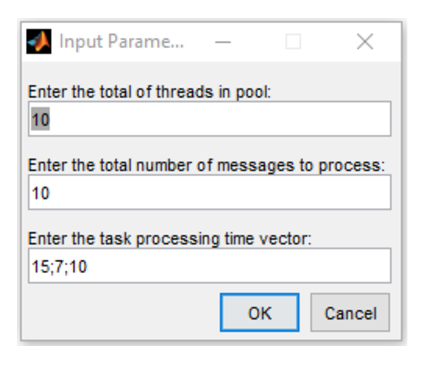
\includegraphics[width=1\linewidth]{./figs/inputs_FIFO.eps}
\end{minipage}
\begin{minipage}[c]{0.49\linewidth}
\centering
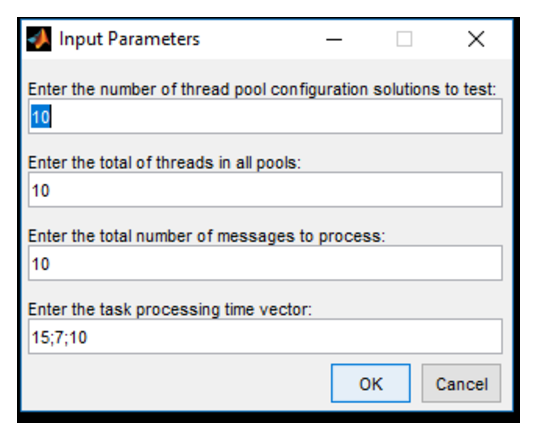
\includegraphics[width=1\linewidth]{./figs/inputs.eps}
\end{minipage}
 \caption{Input interface of the programs.}
\label{fig:inputs}
\end{figure}
Os programas geram uma matriz  com os tempos finais de processamento de cada mensagem por cada uma das tarefas do fluxo. O índice da linha da matriz representa a tarefa executada e o índice da coluna representa a mensagem. O tempo total médio de processamento das mensagens é calculado por meio da média aritmética dos tempos finais das mensagens na última tarefa do fluxo. O programa mostra graficamente a sequência do processamento das mensagens nas tarefas. A Figura~\ref{fig:graphic_sequence} mostra um exemplo dessa sequência. O programa mostra também o tempo total médio de processamento das mensagens, conforme mostrado na Figura~\ref{fig:outputs}. No caso do modelo proposto, mostra a configuração dos pools que resulta no mínimo TTAP. Assim, os parâmetros de saída fornecidos pelo programa são:
\begin{enumerate}
                 \item Matriz de tempos finais de processamento das mensagens.
                 \item Tempo total médio de processamento das mensagens.
                 \item Configuração dos pools de threads ótima ou próxima de ótima. 
\end{enumerate}
\begin{figure}[h]
\centering
 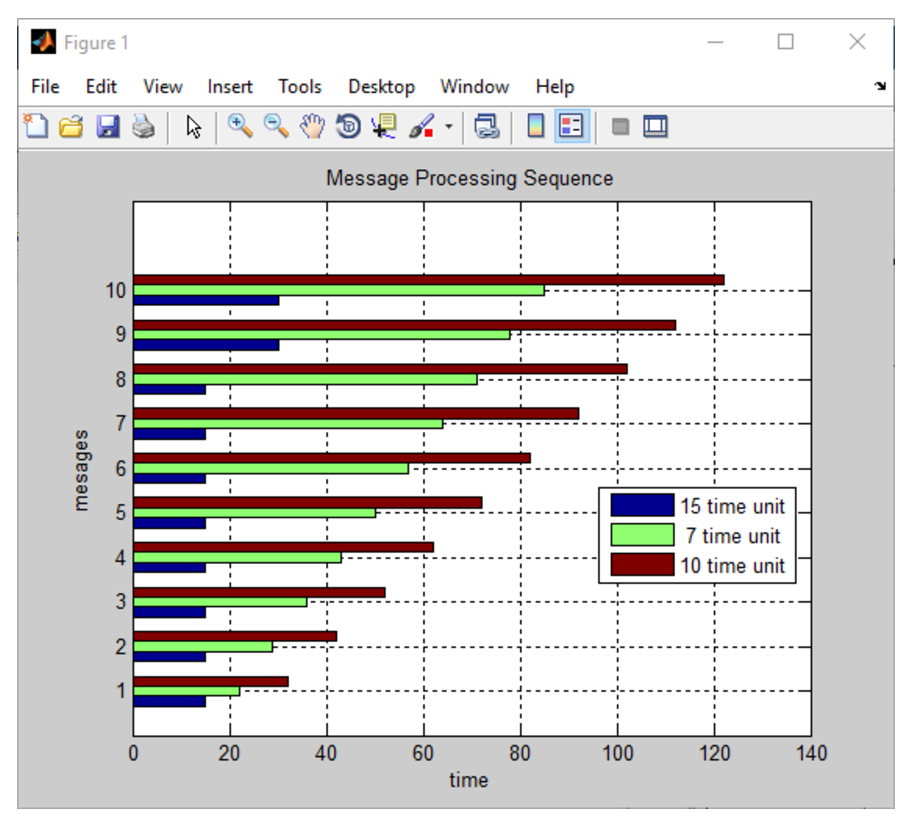
\includegraphics[width=1\linewidth]{./figs/graphic_sequence.eps}
 \caption{Sequence graph example.}
\label{fig:graphic_sequence}
\end{figure}
%
\begin{figure}[h]
\begin{minipage}[c]{0.49\linewidth}
\centering
 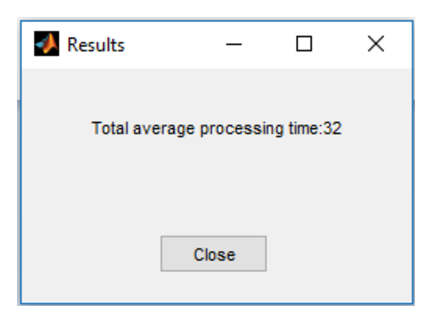
\includegraphics[width=0.8\linewidth]{./figs/outputs_FIFO.eps}
\end{minipage}
\begin{minipage}[c]{0.49\linewidth}
\centering
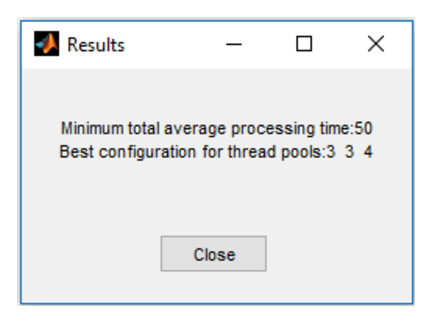
\includegraphics[width=0.8\linewidth]{./figs/outputs_PSO.eps}
\end{minipage}
\caption{Program output interface..}
\label{fig:outputs}
\end{figure}
%==============================================================================
\subsection{Scenarios}
\label{subsec:scenarios}
%==============================================================================
Para testar os programas criados para simulação preliminar do processamento das mensagens no fluxo de um processo de integração, utilizamos um cenário simplificado. Conforme a Figura~\ref{fig:workflow}, o fluxo de tarefas possui três tarefas, cujos tempos de processamento são respectivamente: 15, 7 e 10 unidades de tempo.
\begin{figure}[h]
\centering
 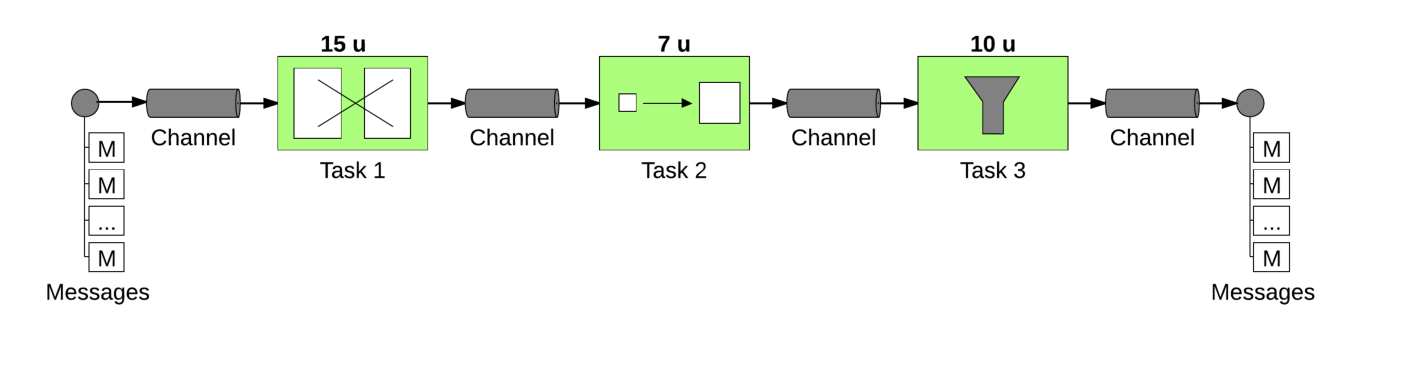
\includegraphics[width=1\linewidth]{./figs/workflow.eps}
 \caption{Workflow sample.}
\label{fig:workflow}
\end{figure}

Criamos vinte quatro cenários diferentes, variando o número total de mensagens a serem processadas: 10, 100, 1000, 10000 mensagens, sendo processadas por pools contendo 3, 4, 5, 6, 7, 8, 9 e 10 threads.
Os parâmetros de entrada utilizados foram:
\begin{itemize}
\item Número total de threads: de 3 a 10.
\item Número total de mensagens a serem processadas: 10, 100, 1000, 10000.
\item Número total de soluções testadas: 100
\item Vetor contendo os tempos de processamentos das tarefas: [15;7;10] 
\end{itemize}
%==============================================================================
\subsection{Actual system}
\label{subsec:actual_system}
%==============================================================================
% - trata-se da execução do "sistema atual" para coletar os valores para as variáveis selecionadas em cada cenário de experimentação
No modelo de agendamento das tarefas com um único pool de threads, todas as threads do pool se encarregam de executar a primeira tarefa, processando toda a carga inicial de mensagens que chega ao canal de entrada da primeira tarefa. Apenas, quando todas as mensagens terminam seu processamento por uma tarefa é que começam a ser processadas pela execução da tarefa subsequente. 

A figura~\ref{fig:graphic_sequence_single} mostra o processamento de mensagens do primeiro cenário, onde a carga inicial é de 10 mensagens, o pool contém 10 threads e o fluxo de processo de integração possui 3 tarefas, cujos tempos de processamento são respectivamente 15, 7 e 10 unidades de tempo. O pool de threads finaliza o processamento das mensagens pela primeira tarefa em 15 unidades de tempo, já que há 10 threads e 10 mensagens para serem processadas. De modo similar, finaliza o processamento das mensagens pela segunda tarefa em 7 unidades de tempos e pela terceira em 10 unidades de tempo. Nesse cenário, o tempo final de processamento de cada uma das mensagens é o mesmo: 32 unidades de tempo. Calculando a média aritmética desses tempos, acha-se que o tempo total médio de processamento das 10 mensagens é de 32 unidades de tempo.

\begin{figure}[h]
\centering
 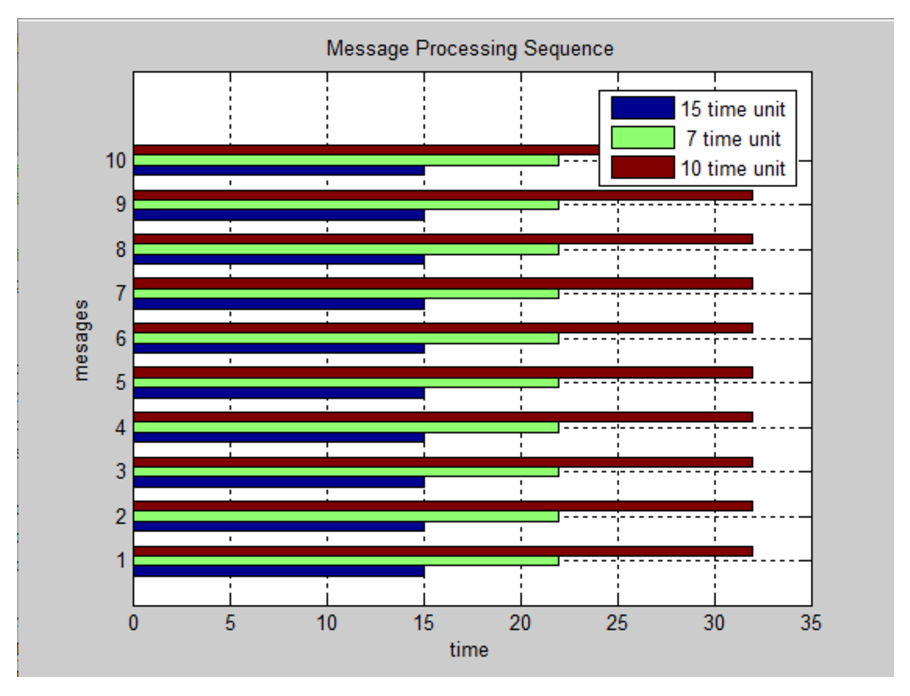
\includegraphics[width=1\linewidth]{./figs/graphic_sequence_single.eps}
 \caption{Processing sequence with single pool.}
\label{fig:graphic_sequence_single}
\end{figure}
%
%==============================================================================
% \subsubsection{Results}
% \label{subsubsec:results_actual_system}
%==============================================================================
%                  - apresentar gráficos/tabelas e, textualmente, descrever os resultados obtidos. Não se deve concluir nada nesta parte
A Figura~\ref{fig:fluxogram_FIFO} retrata o fluxograma do programa desenvolvido para simular esse processamento com cenários com uma carga de entrada com uma maior quantidade de mensagens. A Tabela~\ref{tab:TTAP_single} mostra os valores do tempo total médio de processamento obtidos com cada um dos cenários.
\begin{figure}[h]
\centering
 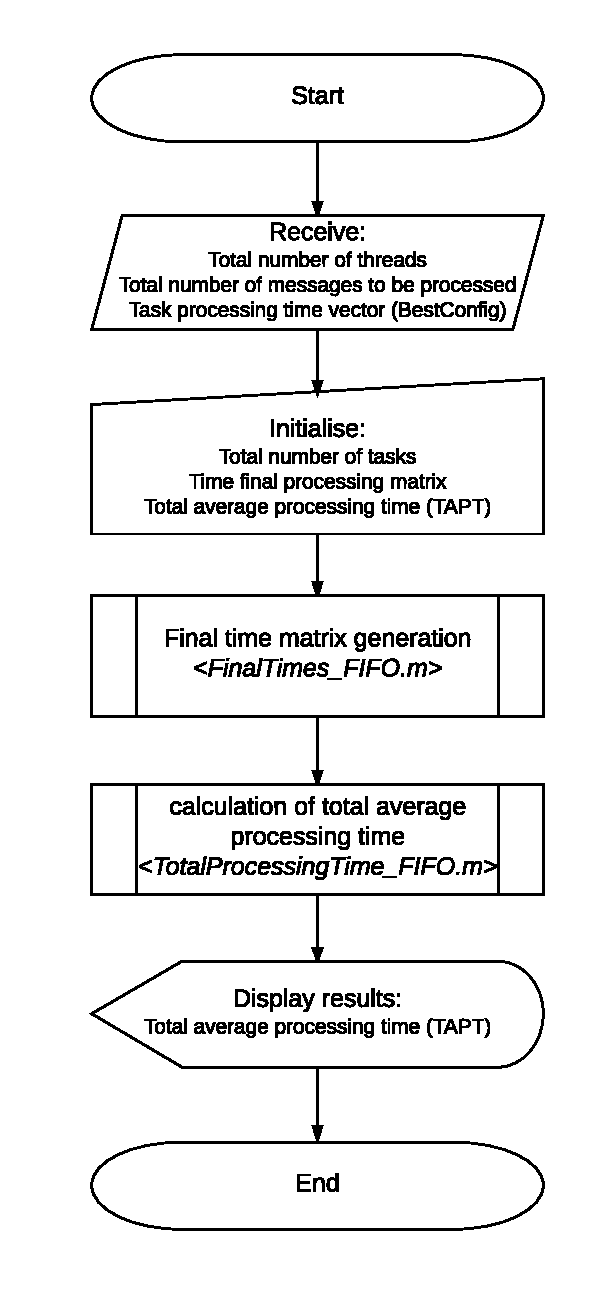
\includegraphics[width=0.7\linewidth]{./figs/fluxogram_FIFO.eps}
 \caption{Scheduling with single thread pool.}
\label{fig:fluxogram_FIFO}
\end{figure}
%
\begin{table}[htb]
\centering
\caption{TTAP with single pool.}
\label{tab:TTAP_single}
\begin{tabular}{cllll}
\hline
\multicolumn{1}{c}{Number of} & \multicolumn{4}{c}{Number of messages} \\
\multicolumn{1}{c}{threads}   & 10         & $10^2$      & $10^3$         & $10^4$    \\ \hline
3                             & 95.30      & 905.03      & 9005.00        & 90005.00        \\
4                             & 72.40      & 680.00      & 6755.00        & 67505.00        \\
5                             & 59.00      & 545.00      & 5405.00        & 54005.00        \\
6                             & 50.60      & 455.00      & 4505.00        & 45005.00        \\
7                             & 43.80      & 390.74      & 3862.14        & 38576.42        \\
8                             & 38.40      & 342.48      & 3380.00        & 33755.00        \\
9                             & 35.20      & 305.02      & 3005.00        & 30005.00        \\
10                            & 32.00      & 275.00      & 2705.00        & 27005.00        \\ \hline
\end{tabular}
\end{table}     

%==============================================================================
\subsection{Optimised system}
\label{subsec:optimised_system}
%==============================================================================
% - trata-se da execução do "sistema otimizado" para coletar os valores para as variáveis selecionadas em cada cenário de experimentação
No modelo de agendamento das tarefas com um múltiplos pools de threads, cada pool só executa a tarefa a qual está dedicado. Dessa forma, a carga inicial de mensagens que chega ao canal da primeira tarefa é processada no pool a ela destinado. Assim, quando uma mensagem termina de ser processada por uma tarefa, já pode ser processada na tarefa subsequente, desde que o haja threads disponíveis no pool dedicado a executar essa próxima tarefa. 

A figura~\ref{fig:graphic_sequence_multiple} mostra o processamento de mensagens no cenário: carga inicial com 10 mensagens; três pools contendo 8, 1, 1 threads, respectivamente; e um fluxo de processo de integração com três tarefas, cujos tempos de processamento são respectivamente 15, 7 e 10 unidades de tempo. Como o pool de threads dedicado a primeira tarefa possui 8 threads, ele finaliza o processamento de 8 mensagens em 15 unidades de tempo e as 2 restantes aguardam 15 unidades de tempo para que esse pool as execute, finalizando o processamento em 30 unidades de tempo. Como o segundo e o terceiro pool só possuem uma thread, O processamento será acrescido de 7 unidades de tempo a cada mensagem na segunda tarefa e em 10 unidades de tempo na terceira. 

\begin{figure}[h]
\centering
 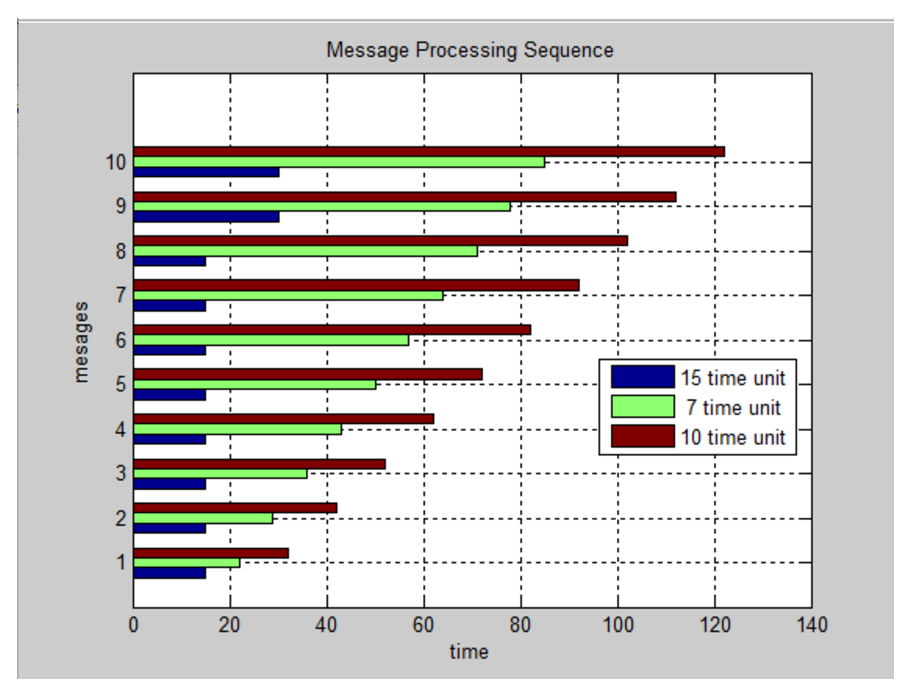
\includegraphics[width=1\linewidth]{./figs/graphic_sequence_multiple.eps}
 \caption{Processing sequence with multiple pools.}
\label{fig:graphic_sequence_multiple}
\end{figure}
%
A Tabela~\ref{tab:TFP} mostra os tempos finais de processamento (TFP) de cada uma das mensagem processadas. Calculando a média aritmética desses tempos, acha-se que o tempo total médio de processamento das 10 mensagens é de 77 unidades de tempo.
%
\begin{table}[htb]
\centering
\caption{TFP with multiple pools.}
\label{tab:TFP}
\begin{tabular}{cllll}
\hline
\multicolumn{1}{c}{Message} & \multicolumn{3}{c}{TFP in task} \\
							  & 1      & 2       & 3            \\ \hline
1                             & 15      & 22      & 32               \\
2                             & 15      & 29      & 42               \\
3                             & 15      & 36      & 52               \\
4                             & 15      & 43      & 62              \\
5                             & 15      & 50      & 72               \\
6                             & 15      & 57      & 82               \\
7                             & 15      & 64      & 92               \\
8                             & 15      & 71      & 102            \\
9                             & 30      & 78      & 112             \\
10                            & 30      & 85      & 122      \\ \hline
\end{tabular}
\end{table} 
% %==============================================================================
% \subsubsection{Results}
% \label{subsubsec:results_optimised_system}
%==============================================================================
%                  - apresentar gráficos/tabelas e, textualmente, descrever os resultados obtidos. Não se deve concluir nada nesta parte.
A Figura~\ref{fig:fluxogram} retrata o fluxograma do programa desenvolvido para simular esse processamento do modelo de múltiplo pools de threads em cenários com uma carga de entrada com uma maior quantidade de mensagens. A Tabela~\ref{tab:best_config} mostra os valores encontrados para as configurações do número de threads em cada pool, utilizando o algoritmo proposto, limitando o número de soluções a 100. A Tabela~\ref{tab:TTAP_multiplo} mostra os valores do tempo total médio de processamento obtidos com essas configurações em cada um dos cenários.
\begin{figure}[h]
\centering
 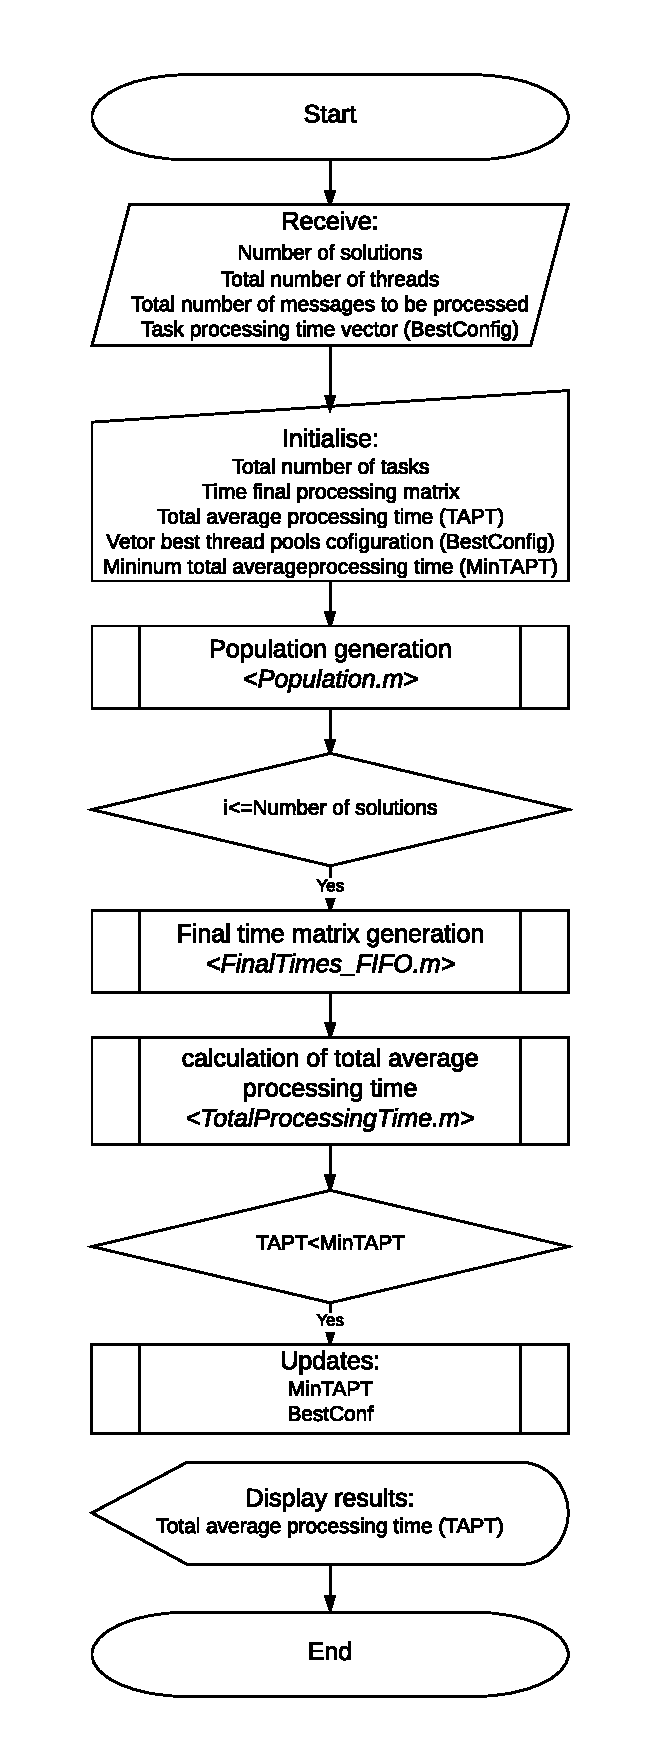
\includegraphics[width=0.8\linewidth]{./figs/fluxogram.eps}
 \caption{Scheduling with multiple pools.}
\label{fig:fluxogram}
\end{figure}
%
\begin{table}[htb]
\centering
\caption{Best configuration of the thread pools.}
\label{tab:best_config}
\begin{tabular}{cllll}
\hline
\multicolumn{1}{c}{Number of}  & \multicolumn{4}{c}{Number of messages} \\
\multicolumn{1}{c}{threads}   & 10           & $10^2$        & $10^3$         & $10^4$          \\ \hline
3                             & [1;1;1]      & [1;1;1]       & [1;1;1]        & [1;1;1]       \\
4                             & [2;1;1]      & [2;1;1]       & [2;1;1]        & [2;1;1]      \\
5                             & [2;1;2]      & [2;1;2]       & [2;1;2]        & [2;1;2]       \\
6                             & [2;2;2]      & [3;1;2]       & [3;1;2]        & [3;1;2]      \\
7                             & [3;2;2]      & [3;2;2]       & [3;2;2]        & [3;2;2]        \\
8                             & [4;2;2]      & [3;2;3]       & [3;2;3]        & [3;2;3]         \\
9                             & [4;2;3]      & [4;2;3]       & [4;2;3]        & [4;2;3]       \\
10                            & [4;2;4]      & [5;2;3]       & [5;2;3]        & [5;2;3]      \\ \hline
\end{tabular}
\end{table}  
%
\begin{table}[htb]
\centering
\caption{TTAP with multiple thread pools.}
\label{tab:TTAP_multiplo}
\begin{tabular}{cllll}
\hline
\multicolumn{1}{c}{Number of} & \multicolumn{4}{c}{Number of messages} \\
\multicolumn{1}{c}{threads}   & 10         & $10^2$       & $10^3$        & $10^4$          \\ \hline
3                             & 99.50      & 774.50       & 7524.50        & 75024.50       \\
4                             & 77.00      & 527.00       & 5027.00        & 50027.00       \\
5                             & 65.50      & 403.00       & 3778.00        & 37528.00       \\
6                             & 62.00      & 378.50       & 3528.50        & 35028.50       \\
7                             & 54.00      & 279.45       & 2529.49        & 25029.49        \\
8                             & 52.00      & 277.00       & 2526.83        & 25026.83        \\
9                             & 47.80      & 216.73       & 1904.24        & 18779.24        \\
10                            & 46.50      & 204.97       & 1779.99        & 175529.99        \\ \hline
\end{tabular}
\end{table}  
%==============================================================================
\subsection{Discussion}
\label{subsec:discussion}
%==============================================================================
%               - analisar os resultados obtidos, buscando explicar valores que possam chamar atenção em cada técnica e comparar os valores obtidos a partir do "optimised model" com aqueles obtidos no "actual system" para avaliar possíveis ganhos.
A Figura~\ref{fig:comparasion} apresenta quatro gráficos comparando o tempo total médio de processamento do modelo utilizando única thread e do modelo utilizado múltiplos pools com o número de threads de cada pool, encontrado pelo algoritmo de otimização. Cada gráfico corresponde a simulação do processamento de 10, 100, 1000 e 10000 mensagens, respectivamente, utilizando pools variando de 3 a 10 threads. 

\begin{figure}[htp]
\centering
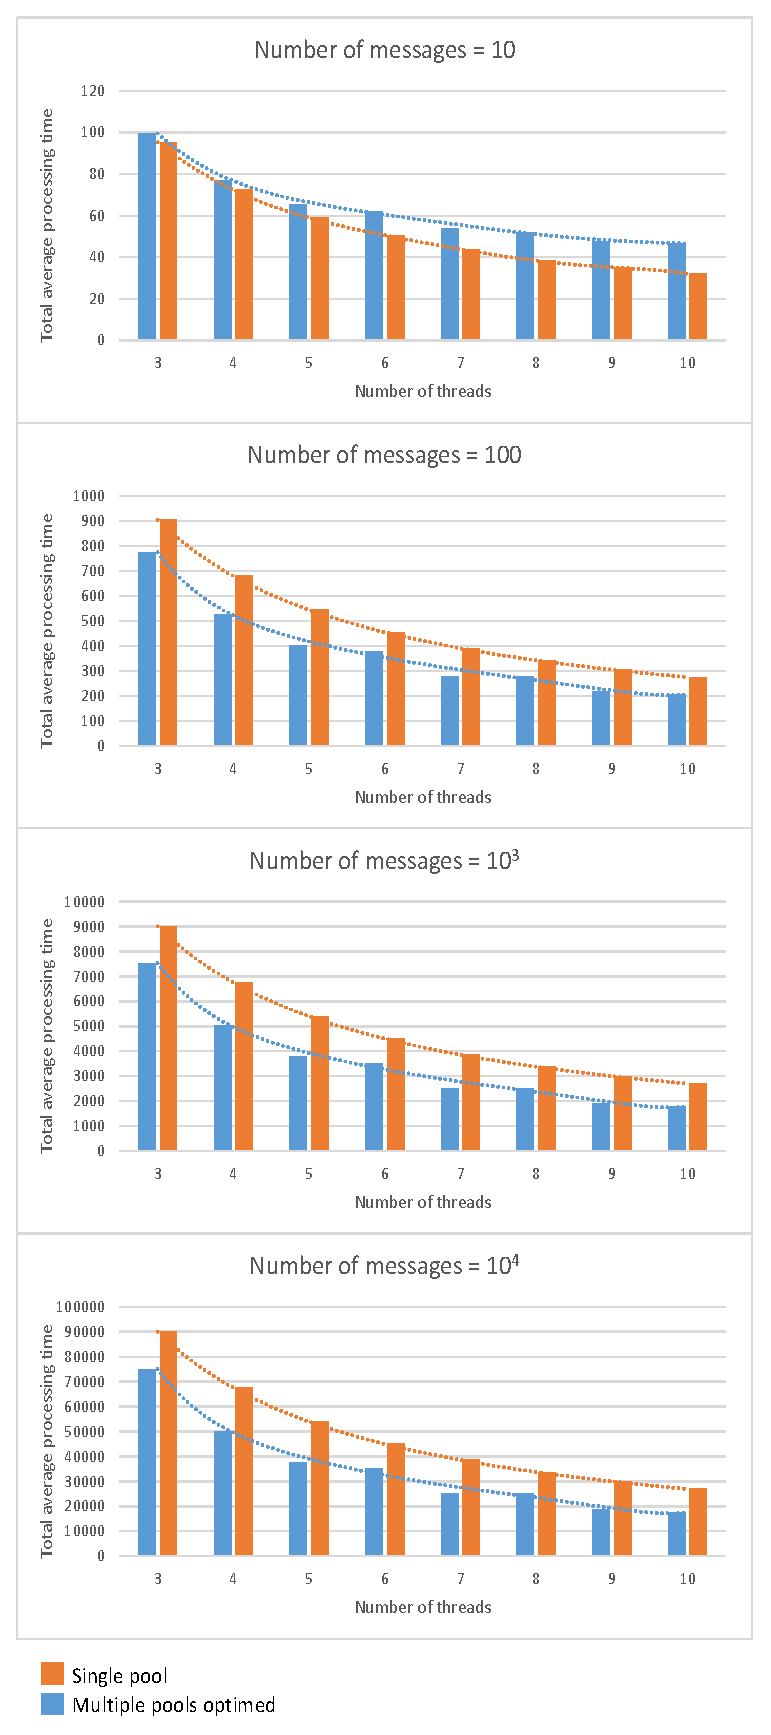
\includegraphics[width=1\linewidth]{./figs/comparasion.eps}
\caption{TTAP with single and multiple threads pools.}
\label{fig:comparasion}
\end{figure}

As barras indicam o valor do TTAP para cada quantidade de threads em ambos os modelos. No primeiro gráfico, com a simulação do processamento de uma carga inicial de 10 mensagens, percebemos que o modelo com o único pool de threads fornece menor TTAP do que o modelo com múltiplos pools e essa diferença aumenta, quando aumentamos o número de threads nos pools. Porém, nos demais gráficos, percebemos que o modelo com múltiplos pools, configurados com o número de threads ótimo, ou perto de ótimo, fornece menor TTAP do que o modelo com único pool. A Tabela~\ref{tab:TTAP_difference} mostra o valor absoluto da diferença entre o TTAP do modelo com único pool e o modelo múltiplos pools, sendo que os valores máximos em cada caso, estão destacados com o símbolo "*". Dos cenários testados, apenas com a carga inicial igual a 10 mensagens, o modelo com único pool foi melhor que o modelo com múltiplos pools de threads, nos demais cenários o modelo proposto apresentou melhores resultados. A diferença atingiu 17478 unidades de tempo a menos no TTAP, utilizando o modelo proposto, quando a carga inicial foi de 10000 mensagens. 
%
\begin{table}[htb]
\centering
\caption{Difference between TTAP.}
\label{tab:TTAP_difference}
\begin{tabular}{cllll}
\hline
\multicolumn{1}{c}{Number of} & \multicolumn{4}{c}{Number of messages} \\
\multicolumn{1}{c}{threads}   & 10         & $10^2$       & $10^3$        & $10^4$          \\ \hline
3                             & 4.20      & 130.53       & 1480.50        & 14980.50       \\
4                             & 4.60      & 153.00*       & 1728.00*        & 17478.00*       \\
5                             & 6.50      & 142.00       & 1627.00        & 16477.00      \\
6                             & 11.40      & 76.56       & 976.50          & 9976.50      \\
7                             & 10.20      & 111.29       & 1332.65        & 13546.93       \\
8                             & 13.60      & 65.48       & 853.17         & 8728.17       \\
9                             & 12.60      & 88.26       & 1100.76        & 11225.76        \\
10                            & 14.50*     & 70.03       & 925.01        & 9475.01        \\ \hline
\end{tabular}
\end{table}  

Os gráficos também apresentam a linha de tendência estatística do TTAP, representada por linhas pontilhadas. A análise por linhas de tendência, também chamada de análise de regressão, permite entender o comportamento de uma variável resposta, por meio de uma equação matemática e assim prever resultados futuros. Uma linha de tendência é mais precisa quanto maior o valor de R-quadrado. R-quadrado é o coeficiente de determinação, número que varia de 0 a 1 e que permite estimar o quanto podemos predizer a variável resposta (TTAP, no nosso caso), a partir da variável preditora (número de threads). Assim, as linhas de tendência apresentadas nos gráficos correspondem a uma equação polinomial, que explica o comportamento do TTAP em relação ao número de threads, permitindo prever o valor de TTAP para uma maior quantidade de threads nos pools. A Tabela~\ref{tab:tendency_line} apresenta essas equações e o R-quadrado correspondente.
%
\begin{table*}[htb]
\centering
\caption{Statistical trend of the TTAP.}
\label{tab:tendency_line}
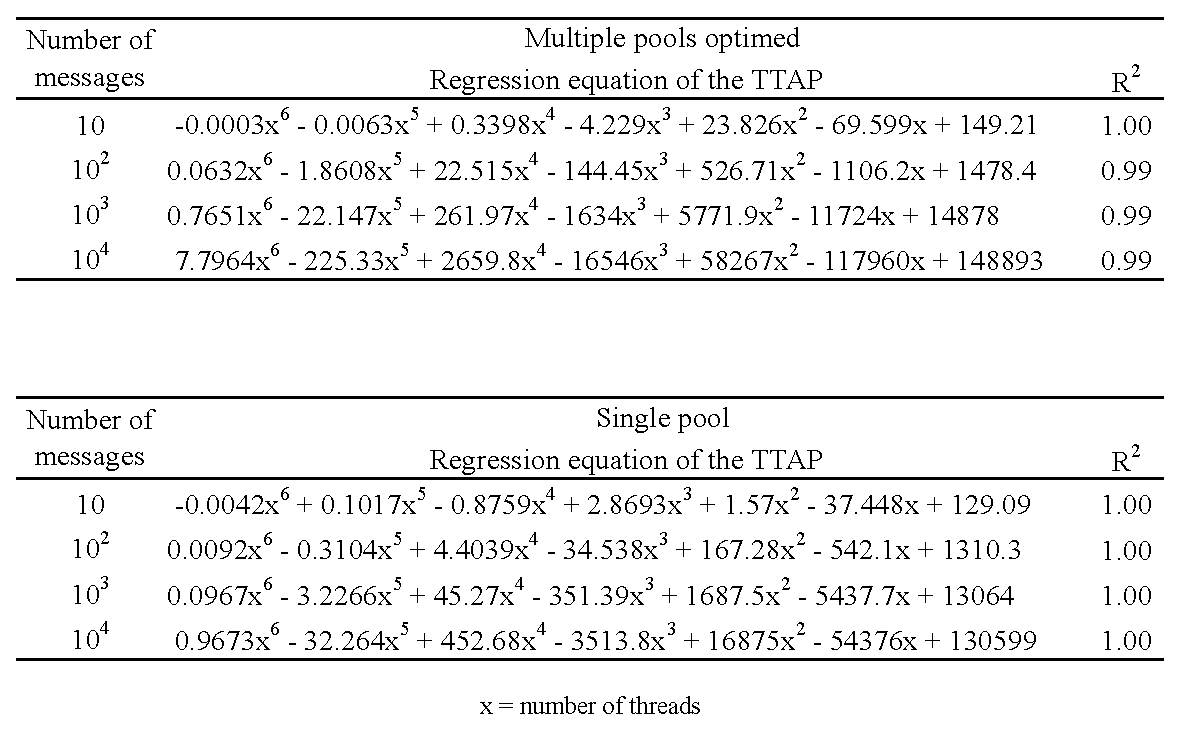
\includegraphics[width=0.7\linewidth]{./figs/equation.eps}
\end{table*}  
%
Assim, as simulações nos cenários apresentados dão indícios de que, a medida que a carga de entrada das mensagens cresce, aumenta a vantagem de se utilizar o modelo com múltiplos pools de threads.


	%==============================================================================
\section{Conclus\~{a}o}
\label{sec:conclusao}
%============================================================================== 
A eficiência dos motores de execução das plataformas de integração está diretamente relacionado com o algoritmo de agendamento das tarefas e a alocação de \emph{threads} para executá-las. Um algoritmo ineficiente leva a um aumento do tempo de execução, degradando assim o desempenho das soluções de integração. Este artigo propõe um algoritmo baseado na meta-heurística \textit{Particle Swarm Optimization} para a alocação de \emph{threads} em motores de execução baseados em filas FIFO. O algoritmo proposto atribui \emph{threads} para as tarefas considerando a complexidade computacional da tarefa e a heterogeneidade na capacidade computacional das \emph{threads}. 
Apesar do PSO localizar de forma rápida a região das boas soluções, é lento no ajuste fino da solução, como acontece em outras técnicas, como no caso dos algoritmos genéticos. Como trabalho futuro, pretende-se implementar esse algoritmo em um motor de execução da plataforma Guaraná para avaliar o ganho de desempenho com distintos casos de uso.

%\bibliographystyle{ACM-Reference-Format}
%\bibliography{sigproc} 

	\begin{small}
		\bibliographystyle{abbrvnat}
		\bibliography{./Bibliography}
	\end{small}
	
\end{document}
